% !TeX program = xelatex
% !TeX encoding = UTF-8
% Spedizione P06 · Dai campioni alla validazione spaziale
% Presentazione della spedizione P06 nella serie planetaria di GeoStat Lab.
% Compilazione: xelatex -interaction=nonstopmode P06_Validazione.tex (due passaggi)
% 27 slide. Diagrammi TikZ, figure vettoriali da R/P06_figure.R, codice R, dati ed esperimenti inclusi.
\RequirePackage{fix-cm}
\documentclass[12pt,aspectratio=1610]{beamer}
\geometry{paperwidth=20cm,paperheight=12.5cm}
\usepackage[italian,provide=*]{babel}
\usepackage{fontspec,adjustbox,tabularx}
\IfFontExistsTF{NimbusSans-Regular.otf}{
\setsansfont{NimbusSans-Regular.otf}[BoldFont=NimbusSans-Bold.otf,ItalicFont=NimbusSans-Italic.otf,BoldItalicFont=NimbusSans-BoldItalic.otf]
\setmainfont{NimbusSans-Regular.otf}[BoldFont=NimbusSans-Bold.otf,ItalicFont=NimbusSans-Italic.otf,BoldItalicFont=NimbusSans-BoldItalic.otf]
}{
\setsansfont{TeX Gyre Heros}
\setmainfont{TeX Gyre Heros}
}
\IfFontExistsTF{DejaVu Sans Mono}{
\setmonofont{DejaVu Sans Mono}[Scale=.88]
}{\setmonofont{Latin Modern Mono}[Scale=.88]}
\usefonttheme{professionalfonts}
\usepackage{amsmath,amssymb,booktabs,array,graphicx,tikz,bookmark}
\usetikzlibrary{calc,positioning,arrows.meta}
\graphicspath{{Figure/}}
\definecolor{Paper}{HTML}{F8F6F1}
\definecolor{Ink}{HTML}{253344}
\definecolor{Navy}{HTML}{15283E}
\definecolor{Quantum}{HTML}{5146A5}
\definecolor{Classical}{HTML}{087C74}
\definecolor{Muted}{HTML}{657180}
\definecolor{Rule}{HTML}{D6DAD9}
\definecolor{Night}{HTML}{112236}
\definecolor{Lilac}{HTML}{ABB5FF}
\definecolor{Mint}{HTML}{72D8C8}
\setbeamercolor{background canvas}{bg=Paper}
\setbeamercolor{normal text}{fg=Ink}
\setbeamertemplate{navigation symbols}{}
\setbeamertemplate{headline}{}
\setbeamertemplate{footline}{}
\setbeamersize{text margin left=0pt,text margin right=0pt}
\hypersetup{colorlinks=true,linkcolor=Classical,urlcolor=Classical,pdfpagemode=UseOutlines,pdfstartview=Fit,
 pdftitle={Spedizione P06 · Dai campioni alla validazione spaziale},pdfauthor={GeoStat Lab · materiali di Marzio De Corato},
 pdfsubject={GeoStat Lab · P06}}
\bookmarksetup{open,openlevel=0,depth=2}
\newsavebox{\BodyBox}
\newsavebox{\SideBox}
\newsavebox{\RecallBox}
\newsavebox{\TitleBox}
\newcommand{\MeasureBox}[2]{\typeout{REVIEWBOX:#1:\the\wd#2:\the\ht#2:\the\dp#2}}

% Revisione completa: diagrammi TikZ, formalismo e box R.
\usepackage[most]{tcolorbox}
\usepackage{listings}
\usetikzlibrary{fit,backgrounds,matrix,decorations.pathreplacing}
\definecolor{GeoA}{HTML}{1D7890}
\definecolor{GeoB}{HTML}{C57E42}
\definecolor{GeoC}{HTML}{7363AA}
\definecolor{GeoTint}{HTML}{F0F4F3}
\lstdefinestyle{GeoR}{language=R,basicstyle=\ttfamily\fontsize{9.2}{12.2}\selectfont,
 keywordstyle=\color{Quantum}\bfseries,commentstyle=\color{Classical},stringstyle=\color{GeoB},
 numbers=left,numberstyle=\tiny\color{Muted},numbersep=4pt,showstringspaces=false,
 columns=fullflexible,keepspaces=true,breaklines=true,xleftmargin=1.15em,
 frame=none,aboveskip=0pt,belowskip=0pt,tabsize=2}
\newsavebox{\PilotLeftBox}
\newsavebox{\PilotRightBox}
\newcommand{\PLabel}[1]{\par{\color{Classical}\bfseries\fontsize{9}{11}\selectfont\MakeUppercase{#1}}\par\vspace{1.8mm}}
\newcommand{\PBody}[1]{\par{\fontsize{11.3}{14.8}\selectfont #1\par}}
\newcommand{\PSmall}[1]{\par{\fontsize{9.8}{13.1}\selectfont #1\par}}
\newcommand{\PCode}[2]{%
\begin{tcolorbox}[enhanced,arc=1.8mm,boxrule=.65pt,
  colback=white,colframe=Classical!75!Navy,colbacktitle=Navy,
  coltitle=white,fonttitle=\bfseries\fontsize{9.6}{12}\selectfont,
  title={#1},left=1.7mm,right=1.3mm,top=1.5mm,bottom=1.3mm,
  before skip=1mm,after skip=1mm]
\lstinputlisting[style=GeoR]{Codice/#2}
\end{tcolorbox}}
\newcommand{\PInfo}[1]{%
\begin{tcolorbox}[enhanced,arc=1.6mm,boxrule=.55pt,colback=GeoTint,
 colframe=Rule!80!Classical,left=2.3mm,right=2.3mm,top=2mm,bottom=2mm,
 before skip=1mm,after skip=1mm]
\PSmall{#1}\end{tcolorbox}}
\tikzset{
 pFlow/.style={draw=Classical!45,fill=white,rounded corners=2mm,
  line width=.7pt,align=center,minimum height=1.1cm,font=\sffamily\fontsize{10}{12}\selectfont},
 pEdge/.style={-{Latex[length=2.3mm]},draw=Classical,line width=.95pt},
 pGroup/.style={draw=Rule,fill=white,rounded corners=2mm,line width=.65pt},
 pDotA/.style={circle,fill=GeoA,inner sep=1.25pt},
 pDotB/.style={circle,fill=GeoB,inner sep=1.25pt},
 pDotC/.style={circle,fill=GeoC,inner sep=1.25pt}
}
\newcommand{\PilotChrome}[4]{%
  \node[anchor=north west,inner sep=0,text width=17.7cm] at ([xshift=.95cm,yshift=-.55cm]current page.north west) {\color{Navy}\bfseries\fontsize{20.6}{24.5}\selectfont #1};
  \node[anchor=north east,inner sep=0] at ([xshift=19.05cm,yshift=-.14cm]current page.north west) {\color{Classical}\fontsize{8}{10}\selectfont\hyperlink{slide2}{#2}};
  \draw[Classical,line width=1.2pt] ([xshift=.95cm,yshift=-1.7cm]current page.north west)--([xshift=2.35cm,yshift=-1.7cm]current page.north west);
  \draw[Rule,line width=.65pt] ([xshift=.95cm,yshift=-10.36cm]current page.north west)--([xshift=19.05cm,yshift=-10.36cm]current page.north west);
  \node[anchor=north west,inner sep=0] at ([xshift=.96cm,yshift=-10.55cm]current page.north west) {\color{Classical}\bfseries\fontsize{9.1}{12}\selectfont DA RICORDARE};
  \node[anchor=north west,inner sep=0,text width=14.3cm] at ([xshift=4.2cm,yshift=-10.53cm]current page.north west) {\color{Ink}\fontsize{10.3}{13.8}\selectfont #4};
  \draw[Rule,line width=.35pt] ([xshift=.95cm,yshift=-11.92cm]current page.north west)--([xshift=19.05cm,yshift=-11.92cm]current page.north west);
  \node[anchor=north west,inner sep=0] at ([xshift=.95cm,yshift=-12.06cm]current page.north west) {\color{Muted}\fontsize{7.7}{9.2}\selectfont Spedizione P06 · Dai campioni alla validazione spaziale};
  \node[anchor=north east,inner sep=0] at ([xshift=19.05cm,yshift=-12.06cm]current page.north west) {\color{Muted}\fontsize{7.7}{9.2}\selectfont #3/27};
}


% Stili comuni per i diagrammi scientifici della revisione completa.
\tikzset{
 pAxis/.style={-{Latex[length=2mm]},draw=Muted,line width=.65pt},
 pNote/.style={font=\sffamily\fontsize{9}{11.5}\selectfont,text=Muted,align=center},
 pLabel/.style={font=\sffamily\fontsize{10}{12.5}\selectfont,text=Ink,align=center}
}
\newsavebox{\FullWideBox}
\setlength{\emergencystretch}{1em}




\newcommand{\PLab}[2]{\par{\color{Classical}\bfseries\fontsize{9}{11}\selectfont
\href{#1}{\MakeUppercase{#2}}}\par\vspace{1.8mm}}

\definecolor{Measure}{HTML}{A05B10}\definecolor{Rose}{HTML}{9B4564}\definecolor{Wash}{HTML}{EAE7F6}\definecolor{Gold}{HTML}{EEC184}
\tikzset{arr/.style={-{Stealth[length=2mm]},line width=.8pt,draw=Classical}}
\newcommand{\Colonna}[2]{\begin{adjustbox}{max totalsize={#1}{7.95cm},valign=t}\begin{minipage}[t]{#1}\raggedright\fontsize{11.3}{14.8}\selectfont #2\end{minipage}\end{adjustbox}}
\begin{document}

\begin{frame}[plain]\hypertarget{slide1}{}\bookmark[level=0,page=1]{Spedizione P06}
\begin{tikzpicture}[remember picture,overlay]
\fill[Night](current page.south west) rectangle(current page.north east);
\IfFileExists{Scena/copertina.jpg}{\node[inner sep=0] at(current page.center){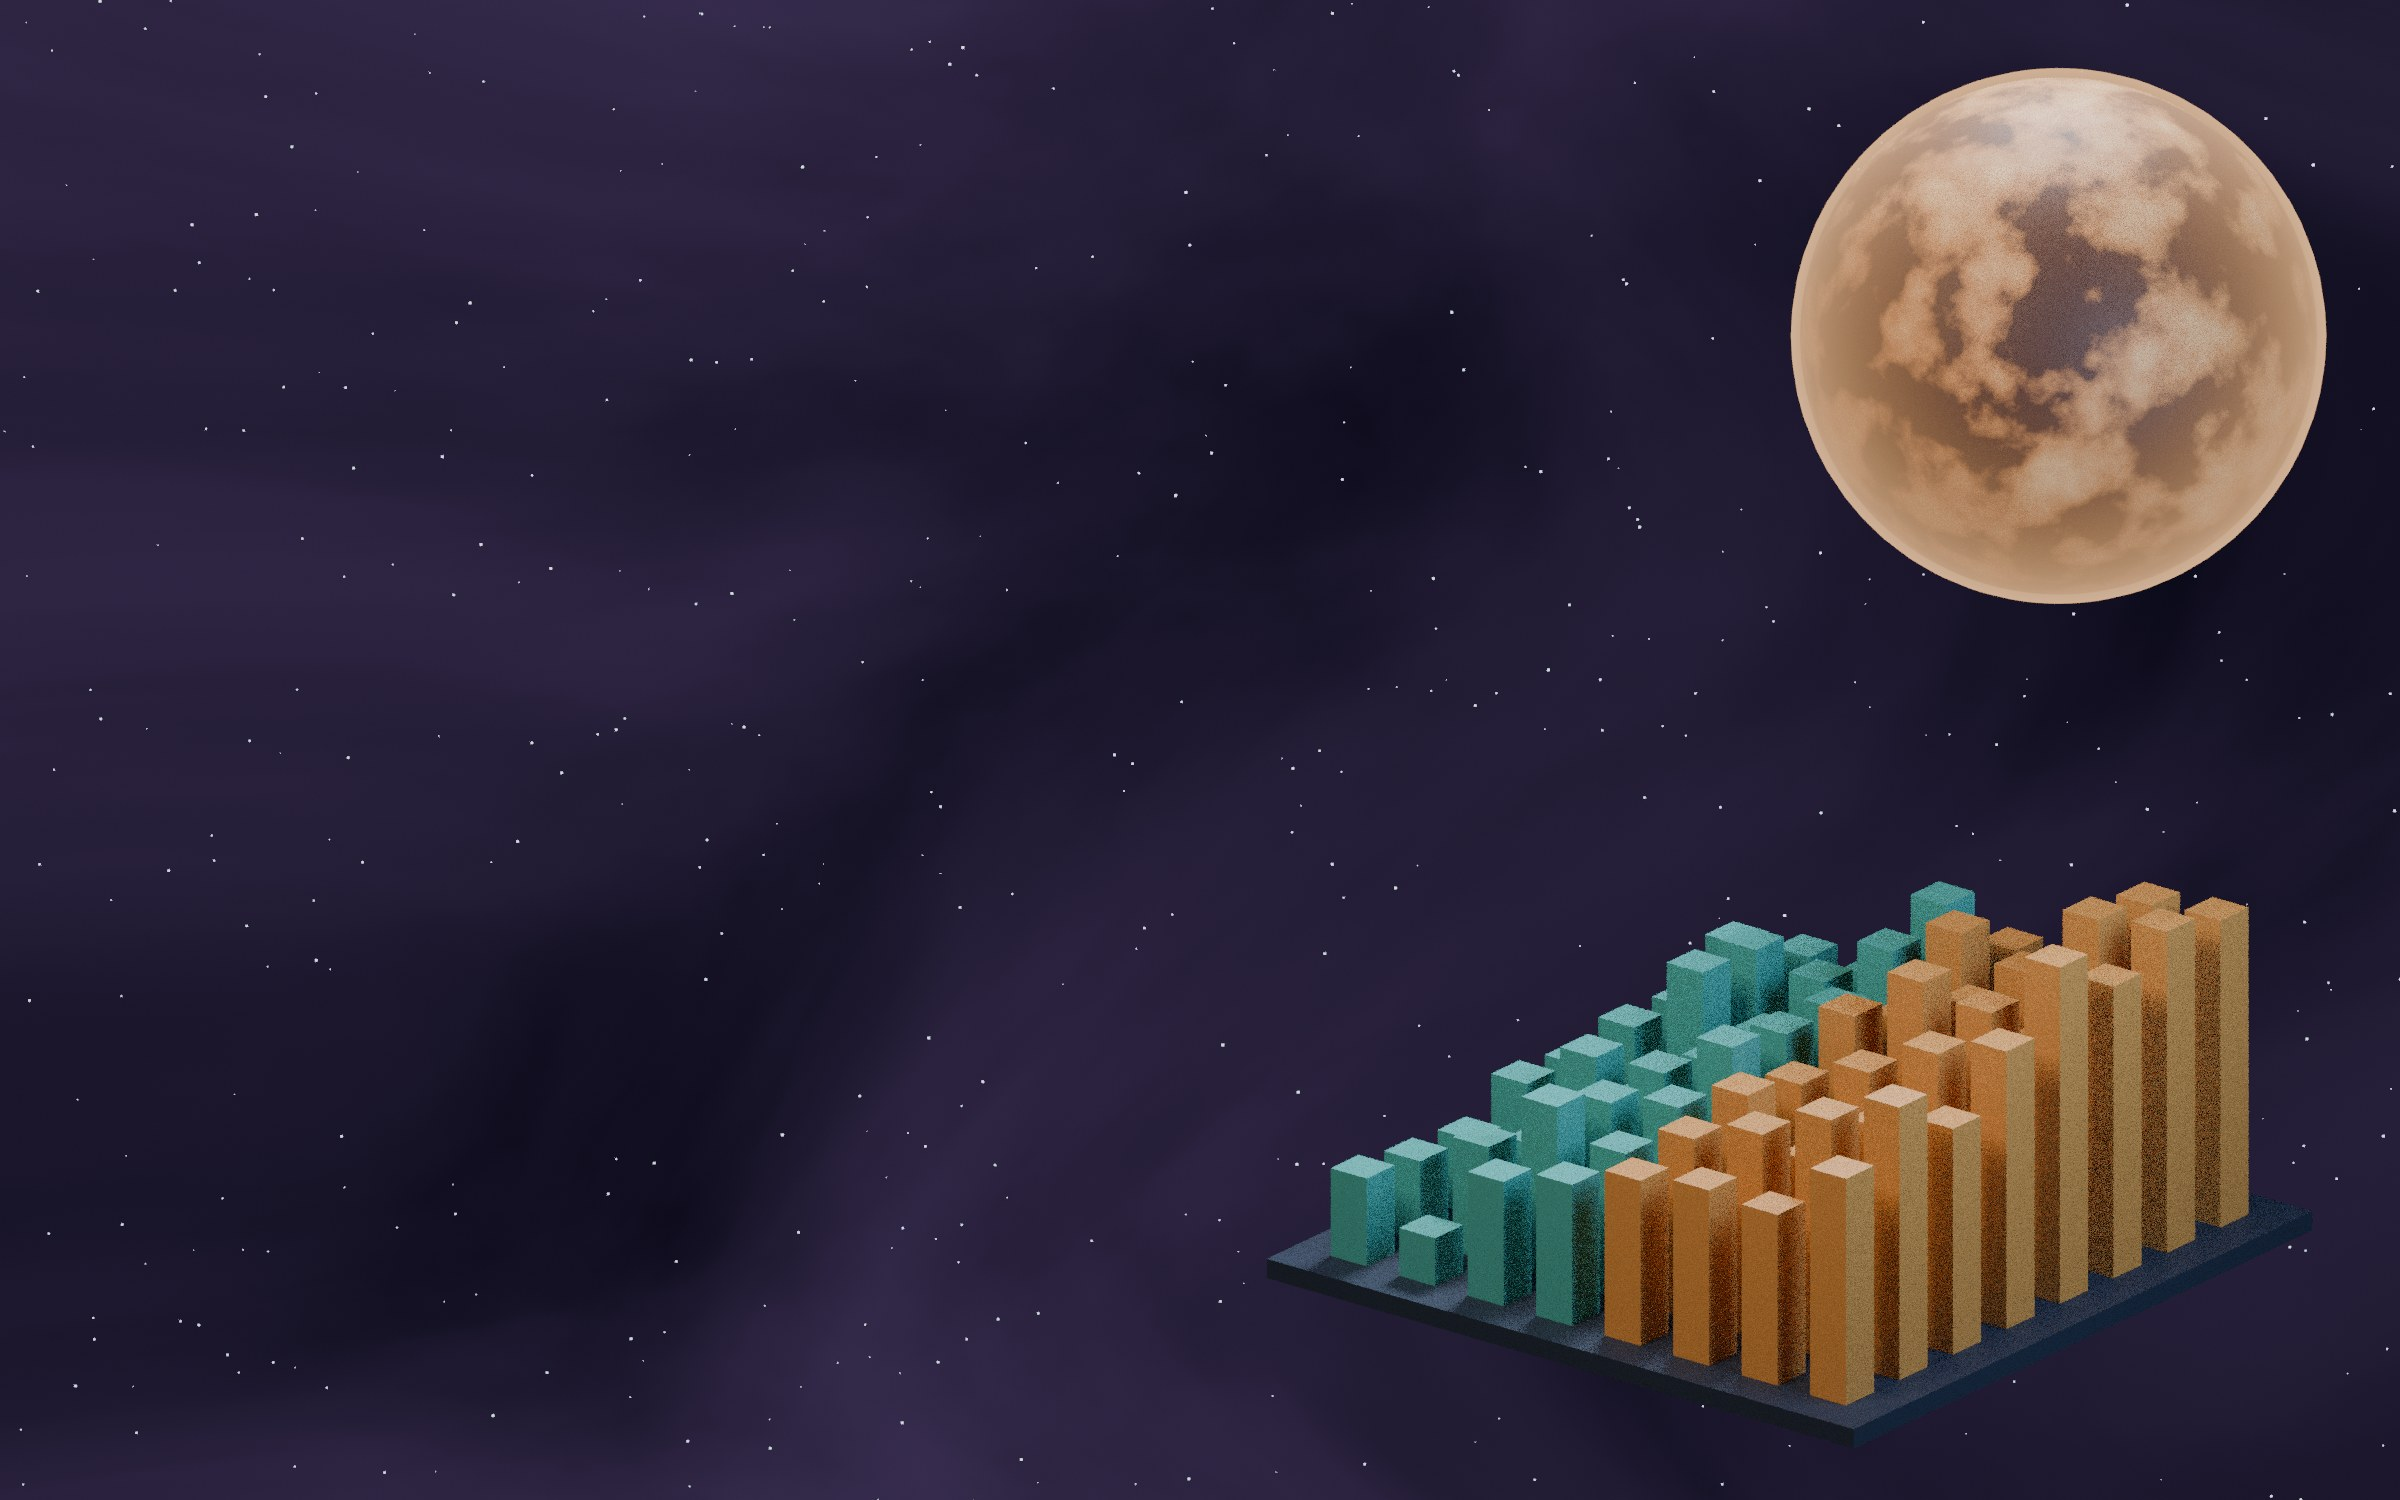
\includegraphics[width=20cm,height=12.5cm]{Scena/copertina.jpg}};}{}
\node[anchor=north west,inner sep=0] at([xshift=1.05cm,yshift=-1.10cm]current page.north west){\color{Mint}\bfseries\fontsize{23}{28}\selectfont SPEDIZIONE P06};
\node[anchor=north west,inner sep=0] at([xshift=1.07cm,yshift=-2.16cm]current page.north west){\color{white}\fontsize{9}{12}\selectfont MACROPROGETTO P06 · SCIENZE DELLA TERRA};
\draw[Mint,line width=1.5pt]([xshift=1.07cm,yshift=-2.78cm]current page.north west)--([xshift=2.6cm,yshift=-2.78cm]current page.north west);
\node[anchor=north west,inner sep=0] at([xshift=1.05cm,yshift=-3.35cm]current page.north west){\begin{minipage}{9.2cm}\raggedright\color{white}\bfseries\fontsize{28.5}{34.5}\selectfont Dai campioni\\alla validazione\\spaziale\end{minipage}};
\node[anchor=north west,inner sep=0] at([xshift=1.07cm,yshift=-7.88cm]current page.north west){\begin{minipage}{8.9cm}\raggedright\color{Lilac}\fontsize{12.2}{17}\selectfont Sessantaquattro siti e un settore escluso\end{minipage}};
\node[anchor=north west,inner sep=0] at([xshift=1.07cm,yshift=-8.70cm]current page.north west){\begin{minipage}{8.9cm}\raggedright\color{white!75}\fontsize{10.3}{14.5}\selectfont Vicinato, permutazioni e trasferimento verso un settore escluso\end{minipage}};
\node[anchor=north west,inner sep=0] at([xshift=1.07cm,yshift=-10.52cm]current page.north west){\color{white}\fontsize{10.5}{14}\selectfont GeoStat Lab · corso di Marzio De Corato};
\node[anchor=north west,inner sep=0] at([xshift=1.07cm,yshift=-11.17cm]current page.north west){\color{Mint}\fontsize{8.8}{11}\selectfont\href{https://creativecommons.org/licenses/by-nc-sa/4.0/}{Impaginazione da Tessera · CC BY-NC-SA 4.0}};
\end{tikzpicture}\end{frame}

\begin{frame}[plain]\hypertarget{slide2}{}
\bookmark[level=1,page=2]{Indice della presentazione}
\begin{tikzpicture}[remember picture,overlay]
\PilotChrome{Indice della presentazione}{PERCORSO}{2}{I titoli dell’indice aprono i capitoli. Il nome del capitolo in alto riporta a questa pagina.}
\node[anchor=north west,inner sep=0] at([xshift=.96cm,yshift=-2.12cm]current page.north west){\Colonna{9.40cm}{\PLabel{Capitoli}
{\fontsize{10.7}{13.5}\selectfont\hyperlink{slide4}{Geometria e osservazioni sintetiche\hfill 4}\par}\vspace{.16cm}
{\fontsize{10.7}{13.5}\selectfont\hyperlink{slide8}{Vicinato e riferimento di permutazione\hfill 8}\par}\vspace{.16cm}
{\fontsize{10.7}{13.5}\selectfont\hyperlink{slide12}{Previsione e verifica nel settore orientale\hfill 12}\par}\vspace{.16cm}
{\fontsize{10.7}{13.5}\selectfont\hyperlink{slide19}{Laboratori della spedizione\hfill 19}\par}\vspace{.16cm}

}};
\node[anchor=north west,inner sep=0] at([xshift=10.85cm,yshift=-2.12cm]current page.north west){\Colonna{8.16cm}{\PLabel{Percorso di lettura}
\PBody{Il percorso definisce geometria e distanze, costruisce il vicinato e il test di permutazione, poi prevede il settore orientale e ne misura gli errori. I laboratori finali riprendono le tre fasi della spedizione.}
\PInfo{Le pagine Scenario A e Confronto riprendono gli esperimenti nel browser con dati sintetici. I valori di partenza del simulatore differiscono da quelli del caso.}
\href{https://marzione00.github.io/Lab_Geo/\#modulo-P06}{\color{Classical}\bfseries Apri la spedizione P06 su GeoStat Lab}
}};
\end{tikzpicture}\end{frame}

\begin{frame}[plain]\hypertarget{slide3}{}
\bookmark[level=1,page=3]{Una struttura spaziale evidente garantisce una buona previsione nel settore orientale escluso?}
\begin{tikzpicture}[remember picture,overlay]
\PilotChrome{{\fontsize{15.3}{19}\selectfont Una struttura spaziale evidente garantisce una buona previsione nel settore orientale escluso?}}{IL CASO GUIDA}{3}{La copertina è una scena illustrativa: le colonne riproducono le concentrazioni, in arancio il settore di verifica.}
\node[anchor=north west,inner sep=0] at([xshift=.96cm,yshift=-2.12cm]current page.north west){\Colonna{9.40cm}{{\centering\resizebox{0.97\linewidth}{!}{\begin{tikzpicture}[x=1cm,y=1cm,every node/.style={font=\sffamily\fontsize{10}{12}\selectfont,text=Ink}]
\draw[draw=Classical,fill=Classical!8,rounded corners=2mm,line width=.7pt] (0,0.00) rectangle (8.6,-0.78);
\node[circle,anchor=center,fill=Classical,inner sep=0,minimum size=.5cm,text=white,font=\sffamily\bfseries\fontsize{9}{10}\selectfont] at (.48,-0.39) {1};
\node[anchor=west,text width=7.4cm,align=left] at (.95,-0.39) {Geometria e osservazioni sintetiche};
\draw[pEdge] (.48,-0.80)--(.48,-1.02);
\draw[draw=Classical,fill=Classical!8,rounded corners=2mm,line width=.7pt] (0,-1.04) rectangle (8.6,-1.82);
\node[circle,anchor=center,fill=Classical,inner sep=0,minimum size=.5cm,text=white,font=\sffamily\bfseries\fontsize{9}{10}\selectfont] at (.48,-1.43) {2};
\node[anchor=west,text width=7.4cm,align=left] at (.95,-1.43) {Vicinato e riferimento di permutazione};
\draw[pEdge] (.48,-1.84)--(.48,-2.06);
\draw[draw=Classical,fill=Classical!8,rounded corners=2mm,line width=.7pt] (0,-2.08) rectangle (8.6,-2.86);
\node[circle,anchor=center,fill=Classical,inner sep=0,minimum size=.5cm,text=white,font=\sffamily\bfseries\fontsize{9}{10}\selectfont] at (.48,-2.47) {3};
\node[anchor=west,text width=7.4cm,align=left] at (.95,-2.47) {Previsione e verifica nel settore orientale};
\draw[pEdge] (.48,-2.88)--(.48,-3.10);
\draw[draw=GeoB,fill=GeoB!8,rounded corners=2mm,line width=.7pt] (0,-3.12) rectangle (8.6,-3.90);
\node[circle,anchor=center,fill=GeoB,inner sep=0,minimum size=.5cm,text=white,font=\sffamily\bfseries\fontsize{9}{10}\selectfont] at (.48,-3.51) {L};
\node[anchor=west,text width=7.4cm,align=left] at (.95,-3.51) {Laboratori della spedizione};
\end{tikzpicture}
}\par}
\PSmall{Capitoli della spedizione; L indica i laboratori conclusivi.}
}};
\node[anchor=north west,inner sep=0] at([xshift=10.85cm,yshift=-2.12cm]current page.north west){\Colonna{8.16cm}{\PLabel{Il caso}
\PBody{Sessantaquattro concentrazioni sintetiche su un reticolo locale con passo di 250 metri permettono due verifiche distinte: l’associazione fra valori vicini e la previsione di un settore orientale escluso dall’adattamento.}
\PInfo{Seguiremo l’indice di Moran con il suo riferimento di permutazione, poi gli errori dell’IDW nella fascia orientale tenuta separata.}
}};
\end{tikzpicture}\end{frame}

\begin{frame}[plain]\hypertarget{slide4}{}
\bookmark[level=0,page=4]{Geometria e osservazioni sintetiche}
\bookmark[level=1,page=4]{La domanda collega struttura e trasferimento}
\begin{tikzpicture}[remember picture,overlay]
\PilotChrome{La domanda collega struttura e trasferimento}{GEOMETRIA E OSSERVAZIONI SINTETICHE}{4}{Il test di associazione spaziale e la verifica predittiva sostengono conclusioni differenti.}
\node[anchor=north west,inner sep=0] at([xshift=.96cm,yshift=-2.12cm]current page.north west){\Colonna{9.40cm}{{\centering\resizebox{0.90\linewidth}{!}{\begin{tikzpicture}[x=1cm,y=-.87cm,every node/.style={font=\fontsize{12.2}{15}\selectfont,text=Ink},arr/.style={-{Stealth[length=2mm]},line width=.8pt,draw=Classical}]\path[use as bounding box] (0,0) rectangle (7.45,6.2);
\draw[draw=Classical,fill=Classical!8,rounded corners=2pt,line width=.7pt] (0.5,0.5) rectangle (6.9,1.8);
\node[anchor=center,text=Ink,font=\fontsize{11.5}{15}\selectfont,text width=6cm,align=center] at (3.7,1.15) {Reticolo e concentrazioni sintetiche};
\draw[arr,draw=Classical] (2,2)--(2,2.8);
\draw[arr,draw=Quantum] (5.4,2)--(5.4,2.8);
\draw[draw=Classical,fill=Classical!8,rounded corners=2pt,line width=.7pt] (0.4,3) rectangle (3.5,4.7);
\node[anchor=center,text=Ink,font=\fontsize{12}{15}\selectfont,text width=2.8cm,align=center] at (1.95,3.85) {Associazione fra vicini};
\draw[draw=Quantum,fill=Quantum!8,rounded corners=2pt,line width=.7pt] (3.9,3) rectangle (7,4.7);
\node[anchor=center,text=Ink,font=\fontsize{11.5}{15}\selectfont,text width=2.8cm,align=center] at (5.45,3.85) {Previsione in un settore escluso};
\node[anchor=center,text=Ink,font=\fontsize{11.5}{15}\selectfont,text width=6.8cm,align=center] at (3.7,5.6) {Due domande, due riferimenti di valutazione};

\end{tikzpicture}}\par}
}};
\node[anchor=north west,inner sep=0] at([xshift=10.85cm,yshift=-2.12cm]current page.north west){\Colonna{8.16cm}{\PBody{Il progetto utilizza sessantaquattro concentrazioni sintetiche collocate su un reticolo locale, per esaminare due problemi distinti: la presenza di associazione fra valori vicini e la capacità di prevedere un settore geografico escluso dall’adattamento. Il primo problema viene formulato attraverso un indice di Moran e un riferimento di permutazione; il secondo richiede previsioni confrontate con valori tenuti separati. Una struttura spaziale evidente può coesistere con errori elevati nel trasferimento, soprattutto quando il settore da prevedere supera il dominio osservato durante l’adattamento.}
}};
\end{tikzpicture}\end{frame}

\begin{frame}[plain]\hypertarget{slide5}{}
\bookmark[level=1,page=5]{Le coordinate locali delimitano il significato metrico}
\begin{tikzpicture}[remember picture,overlay]
\PilotChrome{{\fontsize{15.3}{19}\selectfont Le coordinate locali delimitano il significato metrico}}{GEOMETRIA E OSSERVAZIONI SINTETICHE}{5}{La distanza eredita le unità e le ipotesi geometriche del sistema di coordinate utilizzato.}
\node[anchor=north west,inner sep=0] at([xshift=.96cm,yshift=-2.12cm]current page.north west){\Colonna{9.40cm}{\PBody{Le coordinate x e y variano da zero a 1750 metri con passo di 250 metri, formando otto righe e otto colonne. Le coordinate geografiche incluse nella tabella derivano invece da una costruzione approssimata, della quale va conservata la natura didattica. Le distanze del progetto vengono calcolate sul piano locale metrico, senza attribuirgli automaticamente un sistema UTM reale. Un intervallo numerico plausibile di longitudine e latitudine non certifica datum, accuratezza o provenienza delle posizioni.}
\par\smallskip{\centering\adjustbox{max width=.98\linewidth}{$\displaystyle d_{ij}=\sqrt{(x_i-x_j)^2+(y_i-y_j)^2}$}\par\smallskip}
}};
\node[anchor=north west,inner sep=0] at([xshift=10.85cm,yshift=-2.12cm]current page.north west){\Colonna{8.16cm}{\PInfo{$(x_i,y_i)$ e $(x_j,y_j)$: posizioni dei siti i e j; $d_{ij}$: distanza in metri. Si controllano identificativi, coordinate finite e assenza di duplicati. Metadati di riferimento e protocollo di acquisizione andrebbero documentati, per osservazioni reali, prima di trasformazioni cartografiche.}
}};
\end{tikzpicture}\end{frame}

\begin{frame}[plain]\hypertarget{slide6}{}
\bookmark[level=1,page=6]{La matrice delle distanze}
\begin{tikzpicture}[remember picture,overlay]
\PilotChrome{La matrice delle distanze}{GEOMETRIA E OSSERVAZIONI SINTETICHE}{6}{Le proprietà della matrice verificano la geometria del calcolo e precedono l’interpretazione del campo.}
\node[anchor=north west,inner sep=0] at([xshift=.96cm,yshift=-2.12cm]current page.north west){\Colonna{9.40cm}{\PBody{La matrice D riporta la distanza fra ogni coppia di punti e conserva una diagonale nulla, poiché ogni posizione coincide con sé stessa. La simmetria deriva dalla metrica euclidea, mentre l’assenza di duplicati rende distinti i siti. Questi controlli intercettano errori di costruzione prima che le distanze entrino nei pesi del test e dell’interpolazione. Il significato geologico delle posizioni resta comunque legato alla provenienza dichiarata, che in questo esercizio corrisponde a un dominio sintetico.}
}};
\node[anchor=north west,inner sep=0] at([xshift=10.85cm,yshift=-2.12cm]current page.north west){\Colonna{8.16cm}{\begin{tcolorbox}[enhanced,arc=1.7mm,boxrule=.6pt,colback=white,colframe=Classical!60!Navy,colbacktitle=Navy,coltitle=white,fonttitle=\bfseries\small,title={R · calcolo riproducibile},left=1.7mm,right=1.3mm,top=1.1mm,bottom=1.1mm,before skip=1mm,after skip=1.0mm]\lstinputlisting[style=GeoR,language=R,basicstyle=\ttfamily\fontsize{8.6}{11.4}\selectfont]{Codice/coordinate.R}\end{tcolorbox}
\PLabel{Risultato in R}
\begin{tcolorbox}[colback=GeoTint,colframe=Rule,boxrule=.5pt,arc=1.4mm,left=2mm,right=1mm,top=1mm,bottom=1mm]{\fontsize{8.4}{10.9}\selectfont\ttfamily \mbox{[1]\ \ 250.000\ 2474.874}}\end{tcolorbox}
}};
\end{tikzpicture}\end{frame}

\begin{frame}[plain]\hypertarget{slide7}{}
\bookmark[level=1,page=7]{La carta conserva il supporto puntuale}
\begin{tikzpicture}[remember picture,overlay]
\PilotChrome{La carta conserva il supporto puntuale}{GEOMETRIA E OSSERVAZIONI SINTETICHE}{7}{Supporto della misura e geometria della rappresentazione devono rimanere riconoscibili nella carta.}
\node[anchor=north west,inner sep=0] at([xshift=.96cm,yshift=-2.12cm]current page.north west){\Colonna{9.40cm}{{\centering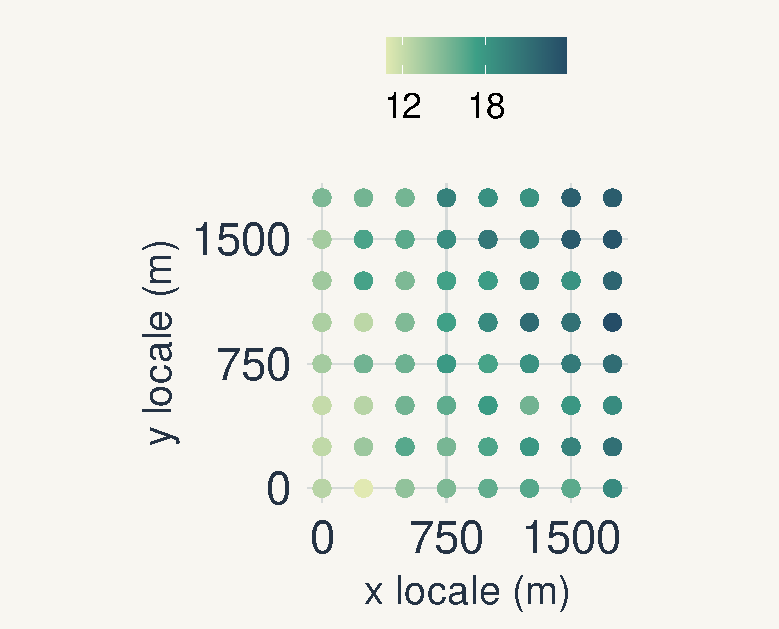
\includegraphics[width=\linewidth,height=6.15cm,keepaspectratio]{Figure/F01.pdf}\par}
\PSmall{Sessantaquattro punti sintetici su un piano locale metrico. Colori: concentrazione in unità arbitrarie.}
}};
\node[anchor=north west,inner sep=0] at([xshift=10.85cm,yshift=-2.12cm]current page.north west){\Colonna{8.16cm}{\PBody{Ogni simbolo rappresenta il valore attribuito a un sito del reticolo, mentre il colore segue una scala comune di concentrazione in unità arbitrarie. Il rapporto unitario fra gli assi conserva le distanze e rende riconoscibile la disposizione dei punti. Gli spazi fra i simboli rimangono privi di un valore osservato: un’eventuale superficie continua richiederebbe un ulteriore modello di interpolazione. La carta descrive quindi la struttura disponibile senza attribuire automaticamente la misura puntuale a tutto il suo intorno.}
}};
\end{tikzpicture}\end{frame}

\begin{frame}[plain]\hypertarget{slide8}{}
\bookmark[level=0,page=8]{Vicinato e riferimento di permutazione}
\bookmark[level=1,page=8]{La soglia di distanza definisce una rete di relazioni}
\begin{tikzpicture}[remember picture,overlay]
\PilotChrome{{\fontsize{15.3}{19}\selectfont La soglia di distanza definisce una rete di relazioni}}{VICINATO E RIFERIMENTO DI PERMUTAZIONE}{8}{L’associazione spaziale viene definita rispetto a una specifica struttura di vicinato.}
\node[anchor=north west,inner sep=0] at([xshift=.96cm,yshift=-2.12cm]current page.north west){\Colonna{9.40cm}{{\centering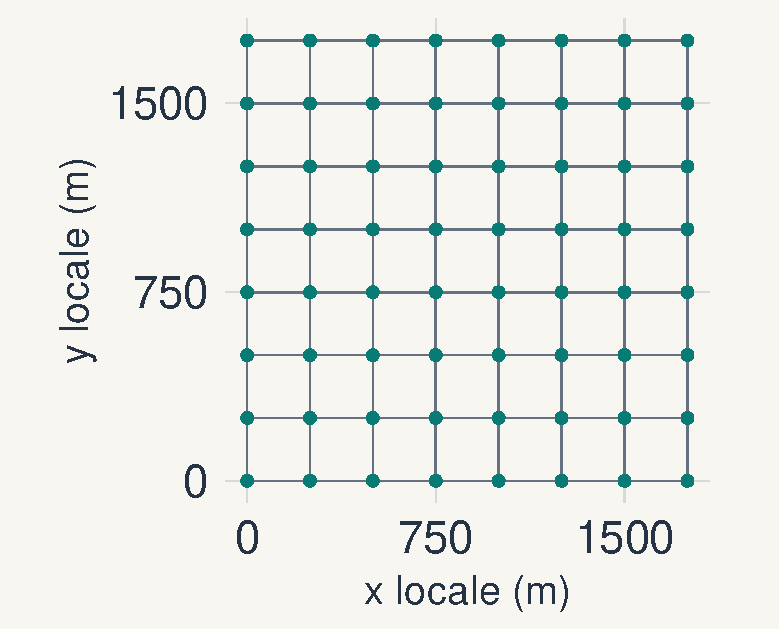
\includegraphics[width=\linewidth,height=6.15cm,keepaspectratio]{Figure/F02.pdf}\par}
\PSmall{$d_{ij}$: distanza in metri. 112 legami non orientati; $S_0=224$ contributi.}
}};
\node[anchor=north west,inner sep=0] at([xshift=10.85cm,yshift=-2.12cm]current page.north west){\Colonna{8.16cm}{\PBody{Due siti sono considerati vicini quando la loro distanza è positiva e non supera 260 metri. Su questo reticolo la regola include i contatti orizzontali e verticali, escludendo quelli diagonali. Si ottengono 112 legami non orientati, che compaiono due volte nella matrice simmetrica dei pesi. La soglia definisce la scala di associazione esaminata e non rappresenta una proprietà universale del processo. Cambiarla modificherebbe il riferimento geometrico dell’indice e richiederebbe una sensibilità dichiarata.}
\par\smallskip{\centering\adjustbox{max width=.98\linewidth}{$\displaystyle w_{ij}=\mathbf1\{0<d_{ij}\leq260\},\qquad S_0=\sum_i\sum_jw_{ij}=224$}\par\smallskip}
}};
\end{tikzpicture}\end{frame}

\begin{frame}[plain]\hypertarget{slide9}{}
\bookmark[level=1,page=9]{L’indice confronta prodotti fra scarti vicini}
\begin{tikzpicture}[remember picture,overlay]
\PilotChrome{L’indice confronta prodotti fra scarti vicini}{VICINATO E RIFERIMENTO DI PERMUTAZIONE}{9}{Segno e grandezza dell’indice dipendono da scarti, dispersione e pesi specificati.}
\node[anchor=north west,inner sep=0] at([xshift=.96cm,yshift=-2.12cm]current page.north west){\Colonna{9.40cm}{{\centering\resizebox{0.90\linewidth}{!}{\begin{tikzpicture}[x=1cm,y=-.87cm,every node/.style={font=\fontsize{12.2}{15}\selectfont,text=Ink},arr/.style={-{Stealth[length=2mm]},line width=.8pt,draw=Classical}]\path[use as bounding box] (0,0) rectangle (7.45,6.2);
\draw[draw=Classical,fill=Classical!8,rounded corners=2pt,line width=.7pt] (0.6,1) rectangle (3.2,2.7);
\node[anchor=center,text=Ink,font=\fontsize{17}{15}\selectfont] at (1.9,1.85) {$v_i>0$};
\draw[draw=Classical,fill=Classical!8,rounded corners=2pt,line width=.7pt] (4.1,1) rectangle (6.7,2.7);
\node[anchor=center,text=Ink,font=\fontsize{17}{15}\selectfont] at (5.4,1.85) {$v_j>0$};
\draw[Quantum,line width=.8pt] (3.2,1.85)--(4.1,1.85);
\node[anchor=center,text=Ink,font=\fontsize{17}{15}\selectfont] at (3.7,3.7) {$w_{ij}v_iv_j>0$};
\node[anchor=center,text=Ink,font=\fontsize{11.5}{15}\selectfont,text width=6.7cm,align=center] at (3.7,5.2) {Scarti concordi contribuiscono positivamente.};

\end{tikzpicture}}\par}
\PSmall{$z_i$: concentrazione; $\bar z$: media; n = 64; $w_{ij}=1$ per $0<d_{ij}\leq260$ m, 0 altrimenti; $S_0=224$.}
}};
\node[anchor=north west,inner sep=0] at([xshift=10.85cm,yshift=-2.12cm]current page.north west){\Colonna{8.16cm}{\PBody{Centrando le concentrazioni rispetto alla media del reticolo, il prodotto fra due scarti è positivo quando entrambi si trovano dalla stessa parte della media. L’indice di Moran riunisce questi prodotti sui legami selezionati e li normalizza mediante dispersione e somma dei pesi. Nel caso osservato vale circa 0,71953. Il valore indica un’associazione positiva rispetto al vicinato binario adottato, mentre la sua interpretazione inferenziale richiede la costruzione di un riferimento coerente con le ipotesi di scambiabilità.}
\par\smallskip{\centering\adjustbox{max width=.98\linewidth}{$\displaystyle v_i=z_i-\overline z,\qquad I=\frac{n}{S_0}\frac{\sum_i\sum_jw_{ij}v_iv_j}{\sum_i v_i^2}$}\par\smallskip}
}};
\end{tikzpicture}\end{frame}

\begin{frame}[plain]\hypertarget{slide10}{}
\bookmark[level=1,page=10]{Le permutazioni conservano siti e valori marginali}
\begin{tikzpicture}[remember picture,overlay]
\PilotChrome{Le permutazioni conservano siti e valori marginali}{VICINATO E RIFERIMENTO DI PERMUTAZIONE}{10}{La distribuzione di permutazione deriva da un’ipotesi sulle assegnazioni ammissibili.}
\node[anchor=north west,inner sep=0] at([xshift=.96cm,yshift=-2.12cm]current page.north west){\Colonna{9.40cm}{{\centering\resizebox{0.90\linewidth}{!}{\begin{tikzpicture}[x=1cm,y=-.87cm,every node/.style={font=\fontsize{12.2}{15}\selectfont,text=Ink},arr/.style={-{Stealth[length=2mm]},line width=.8pt,draw=Classical}]\path[use as bounding box] (0,0) rectangle (7.45,6.2);
\draw[draw=Classical,fill=Classical!8,rounded corners=2pt,line width=.7pt] (0.8,1) rectangle (2.1,2.3);
\node[anchor=center,text=Ink,font=\fontsize{16}{15}\selectfont] at (1.45,1.65) {12};
\draw[draw=Classical,fill=Classical!8,rounded corners=2pt,line width=.7pt] (2.6,1) rectangle (3.9000000000000004,2.3);
\node[anchor=center,text=Ink,font=\fontsize{16}{15}\selectfont] at (3.25,1.65) {18};
\draw[draw=Classical,fill=Classical!8,rounded corners=2pt,line width=.7pt] (4.4,1) rectangle (5.7,2.3);
\node[anchor=center,text=Ink,font=\fontsize{16}{15}\selectfont] at (5.05,1.65) {24};
\draw[arr,draw=Quantum] (3.25,2.7)--(3.25,3.4);
\draw[draw=Quantum,fill=Quantum!8,rounded corners=2pt,line width=.7pt] (0.8,3.8) rectangle (2.1,5.1);
\node[anchor=center,text=Ink,font=\fontsize{16}{15}\selectfont] at (1.45,4.45) {24};
\draw[draw=Quantum,fill=Quantum!8,rounded corners=2pt,line width=.7pt] (2.6,3.8) rectangle (3.9000000000000004,5.1);
\node[anchor=center,text=Ink,font=\fontsize{16}{15}\selectfont] at (3.25,4.45) {12};
\draw[draw=Quantum,fill=Quantum!8,rounded corners=2pt,line width=.7pt] (4.4,3.8) rectangle (5.7,5.1);
\node[anchor=center,text=Ink,font=\fontsize{16}{15}\selectfont] at (5.05,4.45) {18};
\node[anchor=center,text=Ink,font=\fontsize{11}{15}\selectfont,text width=6.8cm,align=center] at (3.7,5.9) {Stesse posizioni, nuova assegnazione dei valori};

\end{tikzpicture}}\par}
}};
\node[anchor=north west,inner sep=0] at([xshift=10.85cm,yshift=-2.12cm]current page.north west){\Colonna{8.16cm}{\PBody{Il riferimento riassegna le concentrazioni alle posizioni fisse e ricalcola l’indice, conservando insieme dei valori e geometria. Questa operazione è pertinente sotto un’ipotesi di scambiabilità delle assegnazioni, che un gradiente spaziale sistematico può rendere scientificamente discutibile come modello nullo. Nel progetto vengono conservati 999 piani di permutazione, così che la distribuzione possa essere ricostruita anche senza ripetere il generatore casuale. L’esito riguarda il riferimento scelto e non identifica il meccanismo fisico che genera la struttura.}
}};
\end{tikzpicture}\end{frame}

\begin{frame}[plain]\hypertarget{slide11}{}
\bookmark[level=1,page=11]{Numero di permutazioni e risoluzione}
\begin{tikzpicture}[remember picture,overlay]
\PilotChrome{Numero di permutazioni e risoluzione}{VICINATO E RIFERIMENTO DI PERMUTAZIONE}{11}{La precisione Monte Carlo e la plausibilità scientifica del riferimento sono componenti distinte del test.}
\node[anchor=north west,inner sep=0] at([xshift=.96cm,yshift=-2.12cm]current page.north west){\Colonna{9.40cm}{{\centering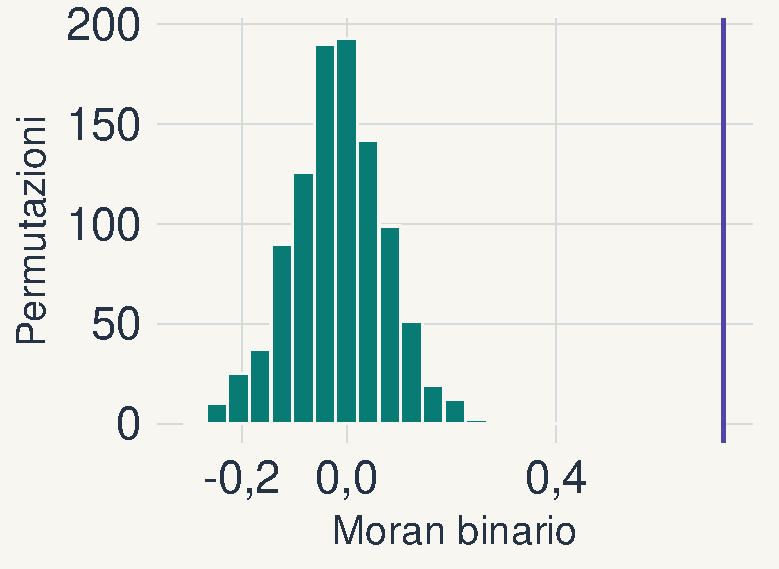
\includegraphics[width=\linewidth,height=6.15cm,keepaspectratio]{Figure/F03.pdf}\par}
\PSmall{$I_b$: indice nella permutazione b; $I_{obs}=0,71953$: indice osservato, in viola. Istogramma: 999 valori permutati.}
}};
\node[anchor=north west,inner sep=0] at([xshift=10.85cm,yshift=-2.12cm]current page.north west){\Colonna{8.16cm}{\PBody{Nessuno dei 999 indici permutati raggiunge quello osservato nella coda positiva. Con la correzione più uno, il p-value Monte Carlo è 0,001, il minimo rappresentabile da questa costruzione. L’assenza di superamenti nel campione simulato non implica una probabilità nulla nel riferimento completo. Aumentare le repliche affina la risoluzione numerica, lasciando immutata l’informazione osservativa del reticolo. La conclusione riguarda l’incompatibilità con l’assegnazione scambiabile considerata e dipende dalla plausibilità scientifica di tale ipotesi.}
\par\smallskip{\centering\adjustbox{max width=.98\linewidth}{$\displaystyle \widehat p=\frac{1+\sum_{b=1}^{999}\mathbf1\{I_b\geq I_{obs}\}}{1000}=0{,}001$}\par\smallskip}
}};
\end{tikzpicture}\end{frame}

\begin{frame}[plain]\hypertarget{slide12}{}
\bookmark[level=0,page=12]{Previsione e verifica nel settore orientale}
\bookmark[level=1,page=12]{La geometria del settore escluso}
\begin{tikzpicture}[remember picture,overlay]
\PilotChrome{La geometria del settore escluso}{PREVISIONE E VERIFICA NEL SETTORE ORIENTALE}{12}{La geometria della separazione determina il tipo di generalizzazione che viene valutato.}
\node[anchor=north west,inner sep=0] at([xshift=.96cm,yshift=-2.12cm]current page.north west){\Colonna{9.40cm}{{\centering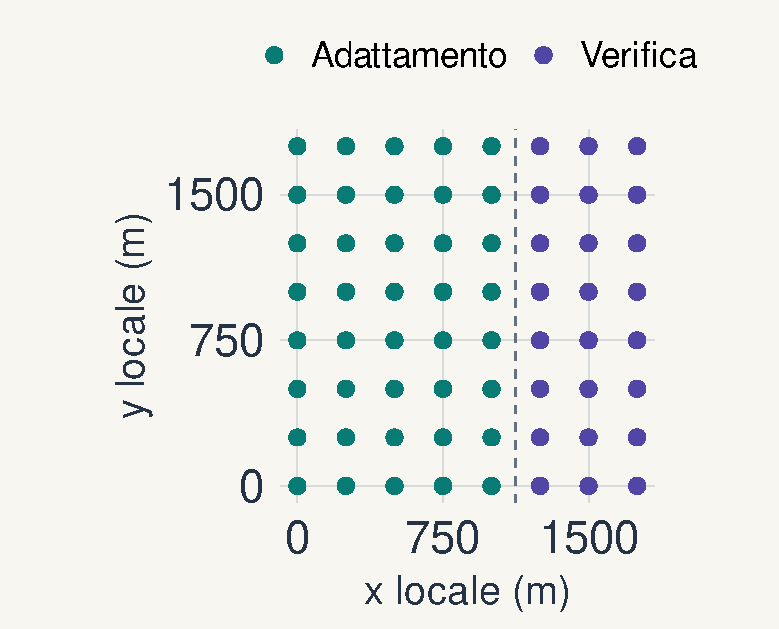
\includegraphics[width=\linewidth,height=6.15cm,keepaspectratio]{Figure/F04.pdf}\par}
\PSmall{Verde: quaranta siti di adattamento; viola: ventiquattro siti orientali separati per la verifica.}
}};
\node[anchor=north west,inner sep=0] at([xshift=10.85cm,yshift=-2.12cm]current page.north west){\Colonna{8.16cm}{\PBody{L’adattamento utilizza i quaranta siti con coordinata x inferiore a 1250 metri, mentre i ventiquattro siti rimanenti costituiscono il settore orientale di verifica. Il valore massimo di x nel train è mille metri, per cui il test oltrepassa la copertura osservata lungo quella direzione. Questa separazione rappresenta un trasferimento spaziale e richiede estrapolazione geografica rispetto ai siti disponibili. Una divisione casuale avrebbe spesso vicini di adattamento attorno ai punti di verifica e risponderebbe a una domanda differente.}
}};
\end{tikzpicture}\end{frame}

\begin{frame}[plain]\hypertarget{slide13}{}
\bookmark[level=1,page=13]{L’IDW costruisce una combinazione convessa locale}
\begin{tikzpicture}[remember picture,overlay]
\PilotChrome{L’IDW costruisce una combinazione convessa locale}{PREVISIONE E VERIFICA NEL SETTORE ORIENTALE}{13}{La positività dei pesi limita la previsione ai valori osservati nei siti utilizzati.}
\node[anchor=north west,inner sep=0] at([xshift=.96cm,yshift=-2.12cm]current page.north west){\Colonna{9.40cm}{{\centering\resizebox{0.90\linewidth}{!}{\begin{tikzpicture}[x=1cm,y=-.87cm,every node/.style={font=\fontsize{12.2}{15}\selectfont,text=Ink},arr/.style={-{Stealth[length=2mm]},line width=.8pt,draw=Classical}]\path[use as bounding box] (0,0) rectangle (7.45,6.2);
\node[anchor=center,text=Quantum,font=\fontsize{20}{15}\selectfont] at (3.7,3) {$s$};
\draw[arr,draw=Classical] (1,1)--(3.4,2.8);
\node[anchor=center,text=Ink,font=\fontsize{13}{15}\selectfont] at (1,1) {1};
\draw[arr,draw=Classical] (6.3,1.2)--(3.4,2.8);
\node[anchor=center,text=Ink,font=\fontsize{13}{15}\selectfont] at (6.3,1.2) {2};
\draw[arr,draw=Classical] (1.2,4.8)--(3.4,2.8);
\node[anchor=center,text=Ink,font=\fontsize{13}{15}\selectfont] at (1.2,4.8) {3};
\draw[arr,draw=Classical] (6.2,4.6)--(3.4,2.8);
\node[anchor=center,text=Ink,font=\fontsize{13}{15}\selectfont] at (6.2,4.6) {4};
\node[anchor=center,text=Ink,font=\fontsize{15}{15}\selectfont,text width=6.6cm,align=center] at (3.7,5.8) {$\lambda_i\geq0,\quad\sum_i\lambda_i=1$};

\end{tikzpicture}}\par}
\PSmall{s: posizione da prevedere; $s_i,z_i$: sito e valore di adattamento; d: distanza in metri, qui positiva. $\lambda_i$: peso normalizzato.}
}};
\node[anchor=north west,inner sep=0] at([xshift=10.85cm,yshift=-2.12cm]current page.north west){\Colonna{8.16cm}{\PBody{La previsione usa pesi inversamente proporzionali al quadrato della distanza dai soli siti di adattamento, normalizzati affinché la loro somma sia uno. La previsione appartiene quindi all’intervallo dei valori disponibili nel train. Quando un gradiente prosegue oltre il settore osservato, questo vincolo può impedire di riprodurre valori più alti presenti nella fascia esclusa. Il calcolo del peso dipende soltanto dalla posizione del punto da prevedere e dai dati ammessi all’adattamento.}
\par\smallskip{\centering\adjustbox{max width=.98\linewidth}{$\displaystyle \lambda_i(s)=\frac{d(s,s_i)^{-2}}{\sum_{j\in train}d(s,s_j)^{-2}},\qquad \widehat z(s)=\sum_{i\in train}\lambda_i(s)z_i$}\par\smallskip}
}};
\end{tikzpicture}\end{frame}

\begin{frame}[plain]\hypertarget{slide14}{}
\bookmark[level=1,page=14]{Il codice esclude le risposte del settore di verifica}
\begin{tikzpicture}[remember picture,overlay]
\PilotChrome{{\fontsize{15.3}{19}\selectfont Il codice esclude le risposte del settore di verifica}}{PREVISIONE E VERIFICA NEL SETTORE ORIENTALE}{14}{La verifica indipendente richiede che i valori da prevedere siano esclusi dalla costruzione dei pesi e della risposta stimata.}
\node[anchor=north west,inner sep=0] at([xshift=.96cm,yshift=-2.12cm]current page.north west){\Colonna{9.40cm}{\PBody{Il frammento percorre i siti orientali e costruisce per ciascuno le distanze dai soli quaranta siti di adattamento. Le concentrazioni orientali entrano soltanto nel calcolo finale degli errori, dopo che le previsioni sono state prodotte. La separazione viene verificata insieme alla finitezza dei risultati e all’appartenenza delle previsioni all’intervallo del train. Una funzione generale gestisce anche il caso di distanza nulla, restituendo il valore del sito coincidente; nella fascia esclusa questo caso non si presenta.}
}};
\node[anchor=north west,inner sep=0] at([xshift=10.85cm,yshift=-2.12cm]current page.north west){\Colonna{8.16cm}{\begin{tcolorbox}[enhanced,arc=1.7mm,boxrule=.6pt,colback=white,colframe=Classical!60!Navy,colbacktitle=Navy,coltitle=white,fonttitle=\bfseries\small,title={R · calcolo riproducibile},left=1.7mm,right=1.3mm,top=1.1mm,bottom=1.1mm,before skip=1mm,after skip=1.0mm]\lstinputlisting[style=GeoR,language=R,basicstyle=\ttfamily\fontsize{8.6}{11.4}\selectfont]{Codice/IDW.R}\end{tcolorbox}
\PLabel{Risultato in R}
\begin{tcolorbox}[colback=GeoTint,colframe=Rule,boxrule=.5pt,arc=1.4mm,left=2mm,right=1mm,top=1mm,bottom=1mm]{\fontsize{8.4}{10.9}\selectfont\ttfamily \mbox{\ \ \ \ \ MAE\ \ \ \ \ RMSE\ }\\\mbox{3.257099\ 3.807826\ }}\end{tcolorbox}
}};
\end{tikzpicture}\end{frame}

\begin{frame}[plain]\hypertarget{slide15}{}
\bookmark[level=1,page=15]{La carta degli errori conserva la loro localizzazione}
\begin{tikzpicture}[remember picture,overlay]
\PilotChrome{{\fontsize{15.3}{19}\selectfont La carta degli errori conserva la loro localizzazione}}{PREVISIONE E VERIFICA NEL SETTORE ORIENTALE}{15}{La posizione e il segno degli errori possono spiegare limiti che una metrica aggregata nasconde.}
\node[anchor=north west,inner sep=0] at([xshift=.96cm,yshift=-2.12cm]current page.north west){\Colonna{9.40cm}{{\centering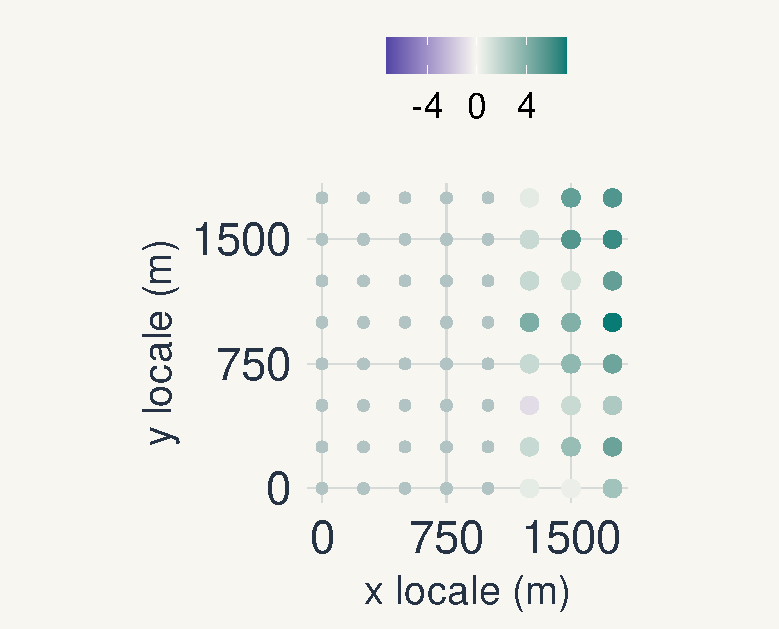
\includegraphics[width=\linewidth,height=6.15cm,keepaspectratio]{Figure/F05.pdf}\par}
\PSmall{Errori osservato meno previsto nella fascia est. Scala divergente centrata sullo zero.}
}};
\node[anchor=north west,inner sep=0] at([xshift=10.85cm,yshift=-2.12cm]current page.north west){\Colonna{8.16cm}{\PBody{Gli errori sono definiti come osservato meno previsto, per cui un valore positivo indica sottostima. La carta mostra dove la previsione si discosti maggiormente dal campo sintetico, mantenendo visibili i siti di adattamento in grigio. La media degli errori è circa 3,175 unità arbitrarie, segnalando una sottostima complessiva nel settore orientale. La localizzazione aiuta a collegare questa direzione dello scarto al gradiente e al vincolo delle combinazioni convesse, evitando di ridurre la diagnosi a un’unica misura aggregata.}
}};
\end{tikzpicture}\end{frame}

\begin{frame}[plain]\hypertarget{slide16}{}
\bookmark[level=1,page=16]{Gli errori vengono quantificati nella scala del campo}
\begin{tikzpicture}[remember picture,overlay]
\PilotChrome{{\fontsize{15.3}{19}\selectfont Gli errori vengono quantificati nella scala del campo}}{PREVISIONE E VERIFICA NEL SETTORE ORIENTALE}{16}{L’associazione spaziale descritta e la capacità di trasferimento valutata rispondono a domande differenti.}
\node[anchor=north west,inner sep=0] at([xshift=.96cm,yshift=-2.12cm]current page.north west){\Colonna{9.40cm}{{\centering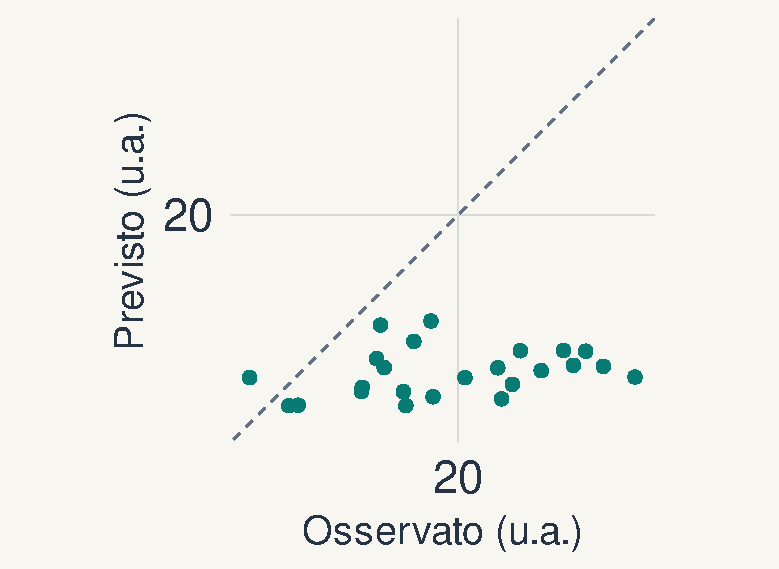
\includegraphics[width=\linewidth,height=6.15cm,keepaspectratio]{Figure/F06.pdf}\par}
\PSmall{Confronto sui ventiquattro siti esclusi. La bisettrice rappresenta previsione esatta.}
}};
\node[anchor=north west,inner sep=0] at([xshift=10.85cm,yshift=-2.12cm]current page.north west){\Colonna{8.16cm}{\PBody{La MAE sul settore orientale è circa 3,257 e la RMSE circa 3,808 unità arbitrarie. Il diagramma osservato–previsto adotta la stessa scala sui due assi e consente di riconoscere le sottostime rispetto alla bisettrice. Queste misure descrivono il trasferimento geografico fissato, mentre il piccolo valore del test di Moran riguarda l’associazione nel reticolo. I due risultati possono dunque coesistere senza contraddizione, poiché una struttura spaziale evidente non garantisce una buona estrapolazione da una parte del dominio.}
}};
\end{tikzpicture}\end{frame}

\begin{frame}[plain]\hypertarget{slide17}{}
\bookmark[level=1,page=17]{La sensibilità della potenza resta esplorativa}
\begin{tikzpicture}[remember picture,overlay]
\PilotChrome{La sensibilità della potenza resta esplorativa}{PREVISIONE E VERIFICA NEL SETTORE ORIENTALE}{17}{Un campione utilizzato per scegliere un parametro cambia ruolo nel procedimento di validazione.}
\node[anchor=north west,inner sep=0] at([xshift=.96cm,yshift=-2.12cm]current page.north west){\Colonna{9.40cm}{{\centering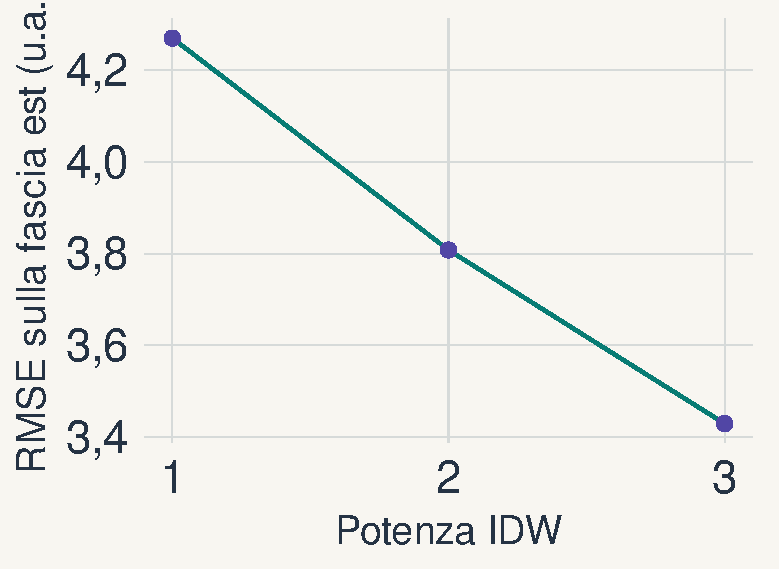
\includegraphics[width=\linewidth,height=6.15cm,keepaspectratio]{Figure/F07.pdf}\par}
\PSmall{Sensibilità descrittiva alla potenza IDW sugli stessi siti orientali; nessuna nuova verifica indipendente.}
}};
\node[anchor=north west,inner sep=0] at([xshift=10.85cm,yshift=-2.12cm]current page.north west){\Colonna{8.16cm}{\PBody{Il confronto delle potenze uno, due e tre rende visibile come una maggiore enfasi sui siti vicini modifichi l’errore nella stessa fascia est. La regola principale rimane quella con potenza due, dichiarata prima della verifica. Se si scegliesse la potenza dopo aver confrontato questi errori, il settore orientale assumerebbe il ruolo di insieme di selezione e servirebbe una nuova area indipendente per la valutazione finale. La figura viene quindi utilizzata per comprendere il metodo e i limiti del disegno.}
}};
\end{tikzpicture}\end{frame}

\begin{frame}[plain]\hypertarget{slide18}{}
\bookmark[level=1,page=18]{Consegna: collegare geometria, test e trasferimento}
\begin{tikzpicture}[remember picture,overlay]
\PilotChrome{{\fontsize{15.3}{19}\selectfont Consegna: collegare geometria, test e trasferimento}}{PREVISIONE E VERIFICA NEL SETTORE ORIENTALE}{18}{La relazione collega la conclusione al riferimento statistico e alla geometria effettivamente valutati.}
\node[anchor=north west,inner sep=0] at([xshift=.96cm,yshift=-2.12cm]current page.north west){\Colonna{9.40cm}{\PBody{La relazione presenta audit metrico, carta dei punti, vicinato, indice con riferimento di permutazione, separazione geografica e mappa degli errori. L’esercizio richiede di spiegare perché un indice elevato possa accompagnarsi a sottostima nel settore orientale, richiamando gradiente e vincoli dei pesi. La conclusione conserva la natura sintetica del campo e indica quali nuove misure territoriali renderebbero più informativo il trasferimento. Codice, piani di permutazione e previsioni per sito permettono di ricostruire ciascun passaggio.}
}};
\node[anchor=north west,inner sep=0] at([xshift=10.85cm,yshift=-2.12cm]current page.north west){\Colonna{8.16cm}{\PInfo{R/P06\_figure.R integra le attività M11\_N01, N07, N14 e N19. Il progetto utilizza il vicinato binario entro 260 metri e 999 permutazioni; i laboratori dichiarano separatamente le proprie numerosità. Le coordinate geografiche approssimate descrivono una costruzione didattica, della quale non si deve inferire una provenienza da rilievo.}
}};
\end{tikzpicture}\end{frame}

\begin{frame}[plain]\hypertarget{slide19}{}
\bookmark[level=0,page=19]{Laboratori della spedizione}
\bookmark[level=1,page=19]{Tre fasi della spedizione nel laboratorio}
\begin{tikzpicture}[remember picture,overlay]
\PilotChrome{Tre fasi della spedizione nel laboratorio}{LABORATORI DELLA SPEDIZIONE}{19}{Gli esperimenti usano campi sintetici; la conclusione sul caso resta quella ottenuta dai sessantaquattro siti.}
\node[anchor=north west,inner sep=0] at([xshift=.96cm,yshift=-2.12cm]current page.north west){\Colonna{9.40cm}{{\centering\resizebox{0.97\linewidth}{!}{\begin{tikzpicture}[x=1cm,y=1cm,every node/.style={font=\sffamily\fontsize{9.2}{11}\selectfont,text=Ink}]
\node[draw=Classical,fill=Classical,rounded corners=2mm,text=white,text width=2.45cm,align=flush center,minimum height=1.55cm,anchor=west,font=\sffamily\bfseries\fontsize{9.2}{11}\selectfont] (f0) at (0,0.00) {1. Definire la geometria};
\node[draw=Classical!60,fill=Classical!6,rounded corners=1.5mm,line width=.6pt,text width=2.8cm,align=flush center,minimum height=1.55cm,anchor=west] (e00) at (2.95,0.00) {Coordinate e metrica delle distanze\\[1pt]{\fontsize{7.6}{9}\selectfont\color{Muted}m11-coordinate}};
\node[draw=Rule,fill=white,rounded corners=1.5mm,line width=.6pt,text width=2.8cm,align=flush center,minimum height=1.55cm,anchor=west] (e01) at (6.10,0.00) {Copertura geografica del campione\\[1pt]{\fontsize{7.6}{9}\selectfont\color{Muted}m11-copertura}};
\draw[pEdge] (f0.east)--(e00.west);
\node[draw=Classical,fill=Classical,rounded corners=2mm,text=white,text width=2.45cm,align=flush center,minimum height=1.55cm,anchor=west,font=\sffamily\bfseries\fontsize{9.2}{11}\selectfont] (f1) at (0,-1.95) {2. Esaminare la struttura};
\draw[pEdge] (f0.south)--(f1.north);
\node[draw=Classical!60,fill=Classical!6,rounded corners=1.5mm,line width=.6pt,text width=2.8cm,align=flush center,minimum height=1.55cm,anchor=west] (e10) at (2.95,-1.95) {Vicinati e matrici dei pesi\\[1pt]{\fontsize{7.6}{9}\selectfont\color{Muted}m11-vicinati}};
\node[draw=Rule,fill=white,rounded corners=1.5mm,line width=.6pt,text width=2.8cm,align=flush center,minimum height=1.55cm,anchor=west] (e11) at (6.10,-1.95) {Dalle coppie al semivariogramma\\[1pt]{\fontsize{7.6}{9}\selectfont\color{Muted}m11-variogramma}};
\draw[pEdge] (f1.east)--(e10.west);
\node[draw=Classical,fill=Classical,rounded corners=2mm,text=white,text width=2.45cm,align=flush center,minimum height=1.55cm,anchor=west,font=\sffamily\bfseries\fontsize{9.2}{11}\selectfont] (f2) at (0,-3.90) {3. Verificare altrove};
\draw[pEdge] (f1.south)--(f2.north);
\node[draw=Classical!60,fill=Classical!6,rounded corners=1.5mm,line width=.6pt,text width=2.8cm,align=flush center,minimum height=1.55cm,anchor=west] (e20) at (2.95,-3.90) {Interpolazione e verifica geografica\\[1pt]{\fontsize{7.6}{9}\selectfont\color{Muted}m11-interpolazione}};
\node[draw=Rule,fill=white,rounded corners=1.5mm,line width=.6pt,text width=2.8cm,align=flush center,minimum height=1.55cm,anchor=west] (e21) at (6.10,-3.90) {Kriging ordinario e incertezza condizionata\\[1pt]{\fontsize{7.6}{9}\selectfont\color{Muted}m11-kriging}};
\draw[pEdge] (f2.east)--(e20.west);
\end{tikzpicture}
}\par}
\PSmall{Fasi della spedizione. Il primo esperimento di ogni fase ha le pagine Scenario A e Confronto.}
}};
\node[anchor=north west,inner sep=0] at([xshift=10.85cm,yshift=-2.12cm]current page.north west){\Colonna{8.16cm}{\PBody{Gli esperimenti ripetono su dati sintetici tre passaggi della spedizione: fissare la metrica delle coordinate, definire il vicinato, verificare un’interpolazione in un’area separata. Ogni fase ha uno scenario di partenza e un confronto con un solo parametro modificato.}
\vspace{.2cm}\PLabel{Altri esperimenti delle fasi}
\PLab{https://marzione00.github.io/Lab_Geo/\#laboratorio/m11-copertura}{Copertura geografica del campione · m11-copertura}
\PLab{https://marzione00.github.io/Lab_Geo/\#laboratorio/m11-variogramma}{Dalle coppie al semivariogramma · m11-variogramma}
\PLab{https://marzione00.github.io/Lab_Geo/\#laboratorio/m11-kriging}{Kriging ordinario e incertezza condizionata · m11-kriging}
}};
\end{tikzpicture}\end{frame}

\begin{frame}[plain]\hypertarget{slide20}{}
\bookmark[level=1,page=20]{Coordinate e metrica delle distanze}
\begin{tikzpicture}[remember picture,overlay]
\PilotChrome{Coordinate e metrica delle distanze}{LABORATORI DELLA SPEDIZIONE}{20}{Verificare la dipendenza della distanza dalle unità degli assi.}
\node[anchor=north west,inner sep=0] at([xshift=.96cm,yshift=-2.12cm]current page.north west){\Colonna{9.40cm}{{\centering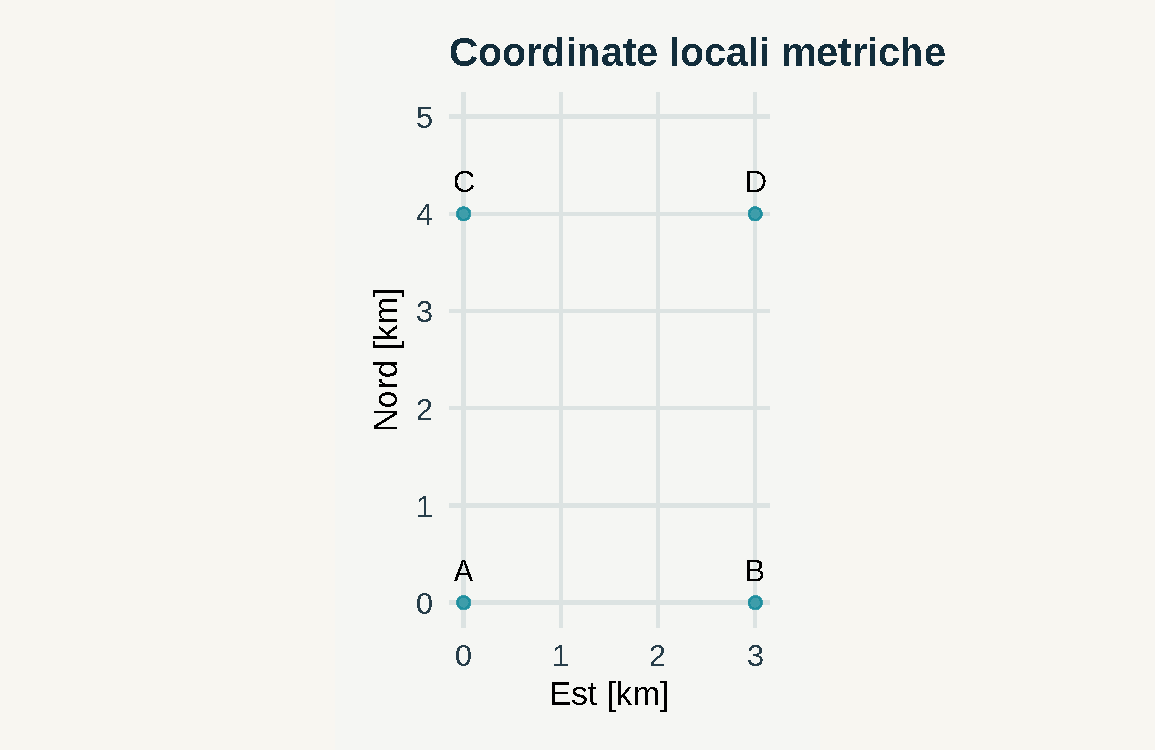
\includegraphics[width=\linewidth,height=5.0cm,keepaspectratio]{Esperimenti/m11-coordinate-A.pdf}\par}
\PSmall{Fattore applicato alla coordinata Est: 1. Seme: 17.}
\PSmall{$x_{i}$ e $y_{i}$ sono le coordinate del punto i nel piano locale; $d_{ij}$ è la distanza fra i e j. Tutte le coordinate e le distanze mostrate sono espresse in chilometri.}
}};
\node[anchor=north west,inner sep=0] at([xshift=10.85cm,yshift=-2.12cm]current page.north west){\Colonna{8.16cm}{\PLabel{Scenario A · simulazione}
\PBody{Le distanze euclidee presuppongono che le coordinate siano espresse in unità compatibili e rappresentino una geometria piana pertinente al problema. I quattro punti dell’esperimento occupano i vertici di un rettangolo, del quale il controllo modifica soltanto l’estensione verso Est. Le distanze riportate permettono di verificare il risultato mediante il teorema di Pitagora.}
\par\smallskip{\centering\adjustbox{max width=.98\linewidth}{$\displaystyle d_{ij}=\sqrt{(x_i-x_j)^2+(y_i-y_j)^2}$}\par\smallskip}
}};
\node[anchor=north east,inner sep=0] at([xshift=17.1cm,yshift=-12.04cm]current page.north west){\fontsize{7.7}{9}\selectfont \href{https://marzione00.github.io/Lab_Geo/\#laboratorio/m11-coordinate}{\color{Classical}\bfseries Apri il laboratorio · m11-coordinate}};
\end{tikzpicture}\end{frame}

\begin{frame}[plain]\hypertarget{slide21}{}
\bookmark[level=1,page=21]{Confronto | Coordinate e metrica delle distanze}
\begin{tikzpicture}[remember picture,overlay]
\PilotChrome{Confronto | Coordinate e metrica delle distanze}{LABORATORI DELLA SPEDIZIONE}{21}{Una distanza euclidea richiede coordinate espresse in unità compatibili.}
\node[anchor=north west,inner sep=0] at([xshift=.96cm,yshift=-2.12cm]current page.north west){\Colonna{9.40cm}{{\centering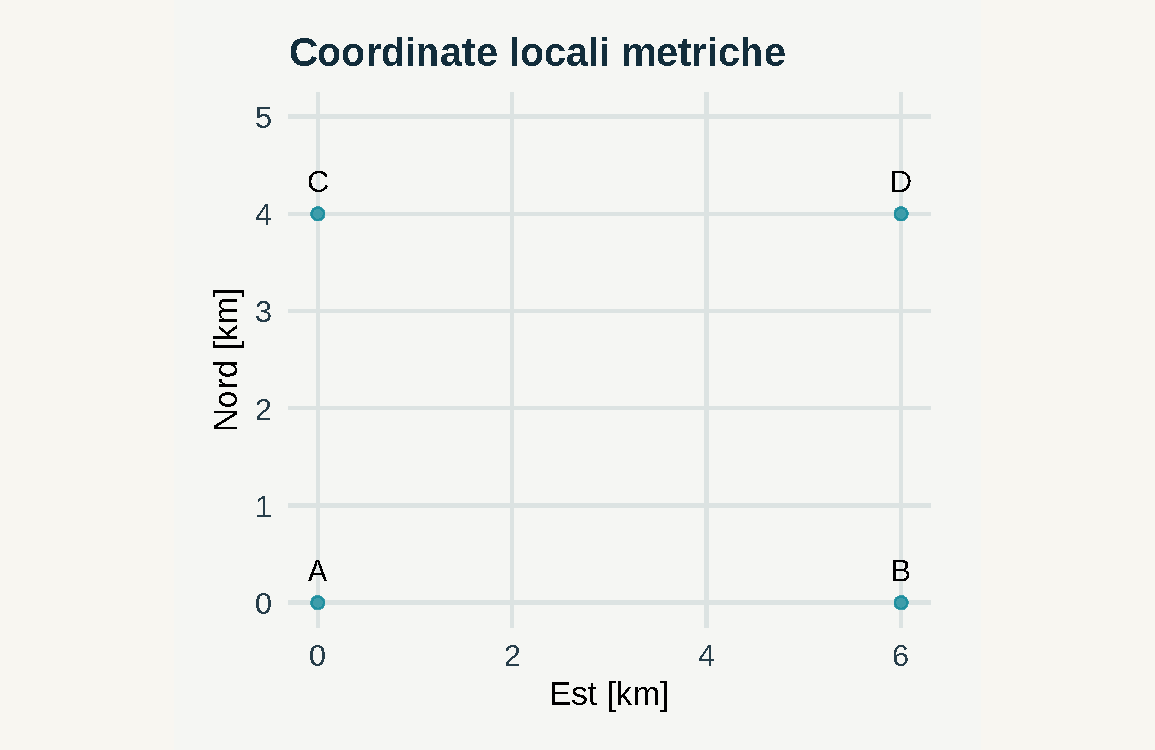
\includegraphics[width=\linewidth,height=5.6cm,keepaspectratio]{Esperimenti/m11-coordinate-B.pdf}\par}
\PSmall{Fattore applicato alla coordinata Est: 1 $\to$ 2. Tutti gli altri parametri e il seme sono fissi.}
}};
\node[anchor=north west,inner sep=0] at([xshift=10.85cm,yshift=-2.12cm]current page.north west){\Colonna{8.16cm}{\PLabel{Confronto fra gli scenari}
{\fontsize{10.2}{12.8}\selectfont\begin{tabular}{@{}>{\raggedright\arraybackslash}p{0.48\linewidth}@{\hspace{.13cm}}>{\raggedright\arraybackslash}p{0.224\linewidth}@{\hspace{.13cm}}>{\raggedright\arraybackslash}p{0.224\linewidth}@{}}\toprule Grandezza & A & B\\[2.3pt]
\midrule 
Distanza A–D [km] & 5 & 7,21\\[2.3pt]
Distanza A–B [km] & 3 & 6\\[2.3pt]
\bottomrule\end{tabular}\par}
\vspace{.25cm}\PBody{Raddoppiando la coordinata Est la distanza A–B passa da 3 a 6 km e la diagonale A–D da 5 a 7,21 km. Un fattore di scala diverso sui due assi altera tutte le distanze che alimentano vicinati e interpolazioni.}
}};
\node[anchor=north east,inner sep=0] at([xshift=17.1cm,yshift=-12.04cm]current page.north west){\fontsize{7.7}{9}\selectfont \href{https://marzione00.github.io/Lab_Geo/\#laboratorio/m11-coordinate}{\color{Classical}\bfseries Apri il laboratorio · m11-coordinate}};
\end{tikzpicture}\end{frame}

\begin{frame}[plain]\hypertarget{slide22}{}
\bookmark[level=1,page=22]{Vicinati e matrici dei pesi}
\begin{tikzpicture}[remember picture,overlay]
\PilotChrome{Vicinati e matrici dei pesi}{LABORATORI DELLA SPEDIZIONE}{22}{Costruire relazioni spaziali a partire da una soglia di distanza.}
\node[anchor=north west,inner sep=0] at([xshift=.96cm,yshift=-2.12cm]current page.north west){\Colonna{9.40cm}{{\centering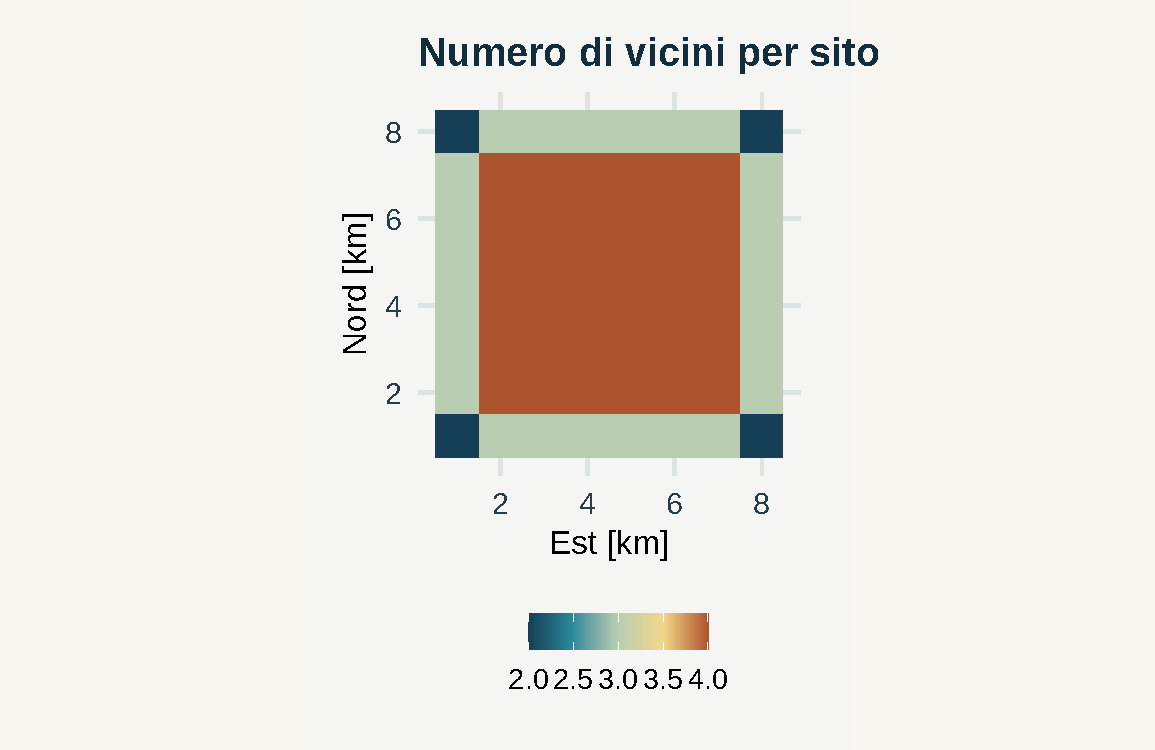
\includegraphics[width=\linewidth,height=6.0cm,keepaspectratio]{Esperimenti/m11-vicinati-A.pdf}\par}
\PSmall{Raggio del vicinato [km]: 1,1. Seme: 17.}
}};
\node[anchor=north west,inner sep=0] at([xshift=10.85cm,yshift=-2.12cm]current page.north west){\Colonna{8.16cm}{\PLabel{Scenario A · simulazione}
\PBody{La costruzione di un vicinato traduce una scelta di scala in una relazione fra siti. Nel reticolo dell’esperimento, due siti distinti sono collegati quando la loro distanza non supera il raggio selezionato. La carta mostra il numero di vicini, permettendo di riconoscere le differenze fra posizioni interne, margini e angoli.}
\par\smallskip{\centering\adjustbox{max width=.98\linewidth}{$\displaystyle w_{ij}=\mathbf1(0<d_{ij}\le r)$}\par\smallskip}
\PSmall{$d_{ij}$ è la distanza fra siti, r il raggio e 1(·) l’indicatore della condizione. La formula definisce i pesi binari; per la normalizzazione ogni riga non nulla viene divisa per la propria somma.}
}};
\node[anchor=north east,inner sep=0] at([xshift=17.1cm,yshift=-12.04cm]current page.north west){\fontsize{7.7}{9}\selectfont \href{https://marzione00.github.io/Lab_Geo/\#laboratorio/m11-vicinati}{\color{Classical}\bfseries Apri il laboratorio · m11-vicinati}};
\end{tikzpicture}\end{frame}

\begin{frame}[plain]\hypertarget{slide23}{}
\bookmark[level=1,page=23]{Confronto | Vicinati e matrici dei pesi}
\begin{tikzpicture}[remember picture,overlay]
\PilotChrome{Confronto | Vicinati e matrici dei pesi}{LABORATORI DELLA SPEDIZIONE}{23}{La matrice dei pesi esprime una scelta di relazione spaziale che precede il calcolo dell’associazione.}
\node[anchor=north west,inner sep=0] at([xshift=.96cm,yshift=-2.12cm]current page.north west){\Colonna{9.40cm}{{\centering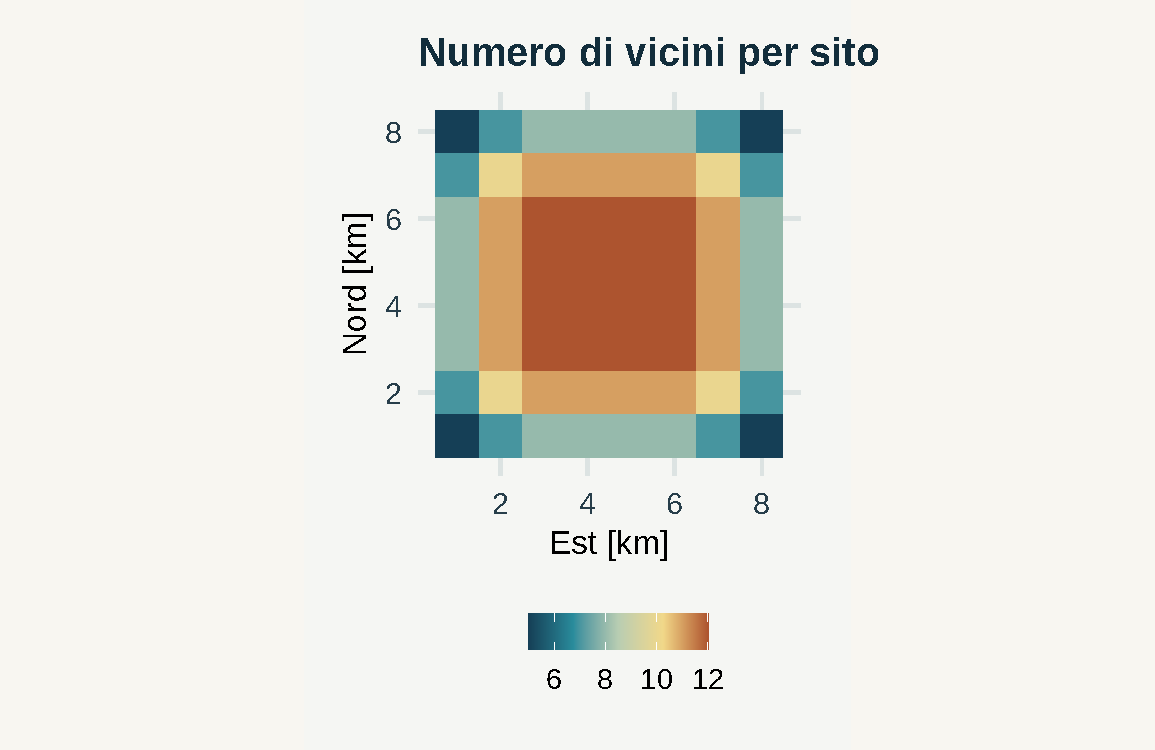
\includegraphics[width=\linewidth,height=5.6cm,keepaspectratio]{Esperimenti/m11-vicinati-B.pdf}\par}
\PSmall{Raggio del vicinato [km]: 1,1 $\to$ 2,0. Tutti gli altri parametri e il seme sono fissi.}
}};
\node[anchor=north west,inner sep=0] at([xshift=10.85cm,yshift=-2.12cm]current page.north west){\Colonna{8.16cm}{\PLabel{Confronto fra gli scenari}
{\fontsize{10.2}{12.8}\selectfont\begin{tabular}{@{}>{\raggedright\arraybackslash}p{0.48\linewidth}@{\hspace{.13cm}}>{\raggedright\arraybackslash}p{0.224\linewidth}@{\hspace{.13cm}}>{\raggedright\arraybackslash}p{0.224\linewidth}@{}}\toprule Grandezza & A & B\\[2.3pt]
\midrule 
Somma dei pesi & 224 & 612\\[2.3pt]
Minimo vicini & 2 & 5\\[2.3pt]
Massimo vicini & 4 & 12\\[2.3pt]
Siti isolati & 0 & 0\\[2.3pt]
\bottomrule\end{tabular}\par}
\vspace{.25cm}\PBody{Con raggio di 2 km la somma dei pesi binari passa da 224 a 612 e il numero di vicini per sito da 2–4 a 5–12. Un indice di Moran calcolato su questa rete descrive una scala spaziale diversa.}
}};
\node[anchor=north east,inner sep=0] at([xshift=17.1cm,yshift=-12.04cm]current page.north west){\fontsize{7.7}{9}\selectfont \href{https://marzione00.github.io/Lab_Geo/\#laboratorio/m11-vicinati}{\color{Classical}\bfseries Apri il laboratorio · m11-vicinati}};
\end{tikzpicture}\end{frame}

\begin{frame}[plain]\hypertarget{slide24}{}
\bookmark[level=1,page=24]{Interpolazione e verifica geografica}
\begin{tikzpicture}[remember picture,overlay]
\PilotChrome{Interpolazione e verifica geografica}{LABORATORI DELLA SPEDIZIONE}{24}{Confrontare IDW e un riferimento mediante campioni separati nello spazio.}
\node[anchor=north west,inner sep=0] at([xshift=.96cm,yshift=-2.12cm]current page.north west){\Colonna{9.40cm}{{\centering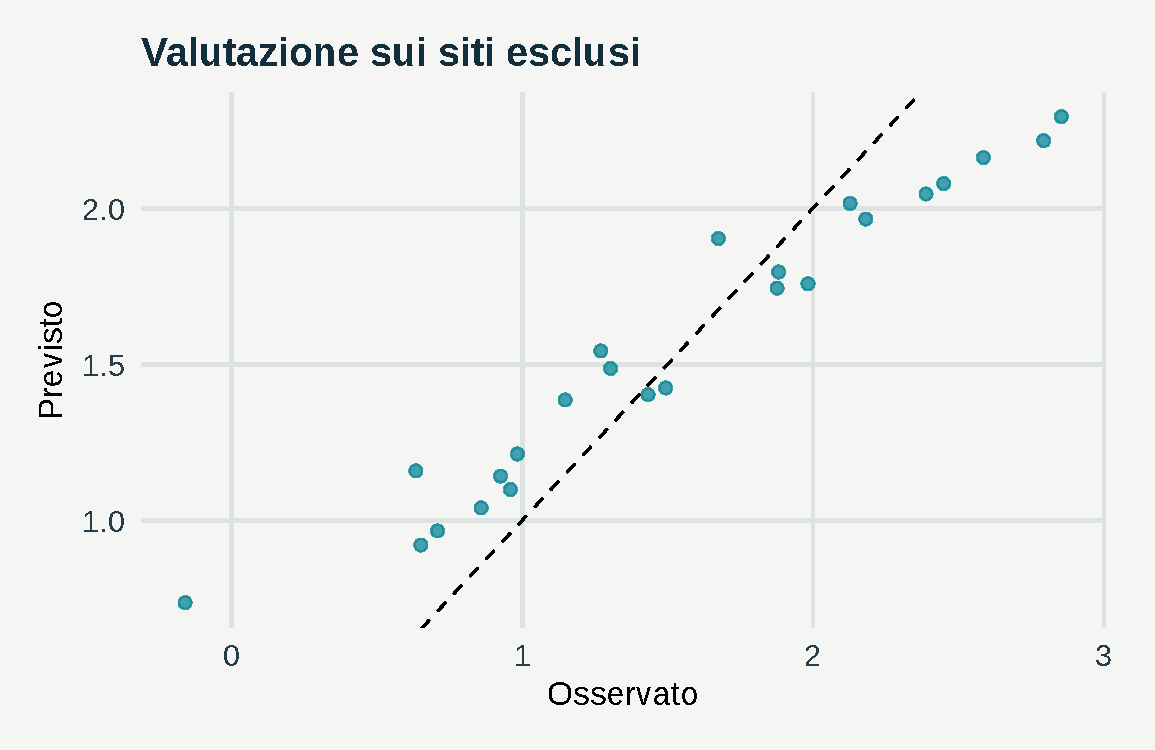
\includegraphics[width=\linewidth,height=5.0cm,keepaspectratio]{Esperimenti/m11-interpolazione-A.pdf}\par}
\PSmall{Separazione: Casuale. Seme: 17.}
\PSmall{$z_{i}$ è il valore osservato nel sito i, d(s,$s_{i}$) la distanza dalla posizione richiesta e p la potenza IDW. I pesi normalizzati sommano a uno; con p=0 le osservazioni non coincidenti ricevono uguale peso.}
}};
\node[anchor=north west,inner sep=0] at([xshift=10.85cm,yshift=-2.12cm]current page.north west){\Colonna{8.16cm}{\PLabel{Scenario A · simulazione}
\PBody{L’interpolazione a distanza inversa combina le misure attribuendo maggiore peso ai siti vicini alla posizione richiesta. L’esponente controlla quanto rapidamente diminuisca il contributo con la distanza. L’esperimento esclude alcuni siti dalla stima e confronta le previsioni con i valori mantenuti per la verifica, affiancando il riferimento costituito dalla media del campione di addestramento.}
\par\smallskip{\centering\adjustbox{max width=.98\linewidth}{$\displaystyle \widehat z(s)=\frac{\sum_i d(s,s_i)^{-p}z_i}{\sum_i d(s,s_i)^{-p}}$}\par\smallskip}
}};
\node[anchor=north east,inner sep=0] at([xshift=17.1cm,yshift=-12.04cm]current page.north west){\fontsize{7.7}{9}\selectfont \href{https://marzione00.github.io/Lab_Geo/\#laboratorio/m11-interpolazione}{\color{Classical}\bfseries Apri il laboratorio · m11-interpolazione}};
\end{tikzpicture}\end{frame}

\begin{frame}[plain]\hypertarget{slide25}{}
\bookmark[level=1,page=25]{Confronto | Interpolazione e verifica geografica}
\begin{tikzpicture}[remember picture,overlay]
\PilotChrome{Confronto | Interpolazione e verifica geografica}{LABORATORI DELLA SPEDIZIONE}{25}{Il test geografico misura il trasferimento alla regione esclusa dall’adattamento.}
\node[anchor=north west,inner sep=0] at([xshift=.96cm,yshift=-2.12cm]current page.north west){\Colonna{9.40cm}{{\centering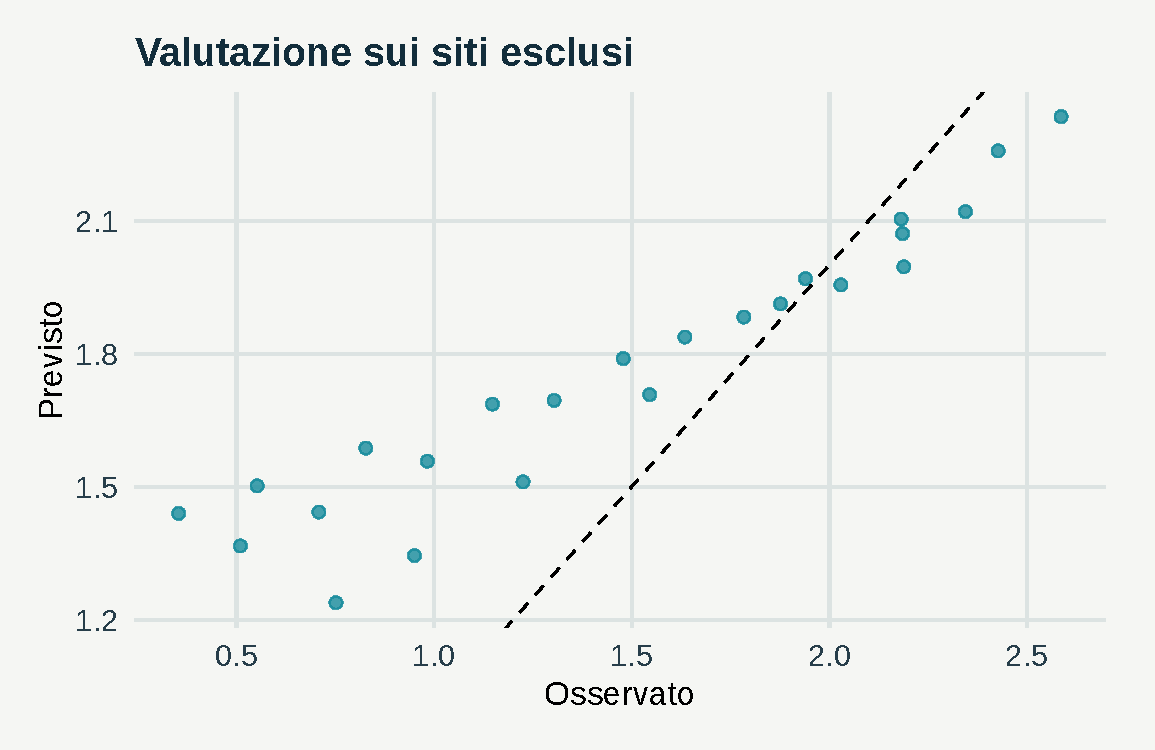
\includegraphics[width=\linewidth,height=5.6cm,keepaspectratio]{Esperimenti/m11-interpolazione-B.pdf}\par}
\PSmall{Separazione: Casuale $\to$ Settore orientale escluso. Tutti gli altri parametri e il seme sono fissi.}
}};
\node[anchor=north west,inner sep=0] at([xshift=10.85cm,yshift=-2.12cm]current page.north west){\Colonna{8.16cm}{\PLabel{Confronto fra gli scenari}
{\fontsize{10.2}{12.8}\selectfont\begin{tabular}{@{}>{\raggedright\arraybackslash}p{0.48\linewidth}@{\hspace{.13cm}}>{\raggedright\arraybackslash}p{0.224\linewidth}@{\hspace{.13cm}}>{\raggedright\arraybackslash}p{0.224\linewidth}@{}}\toprule Grandezza & A & B\\[2.3pt]
\midrule 
Siti di stima & 40 & 40\\[2.3pt]
Siti di test & 24 & 24\\[2.3pt]
RMSE IDW & 0,342 & 0,482\\[2.3pt]
RMSE media di training & 0,767 & 0,667\\[2.3pt]
\bottomrule\end{tabular}\par}
\vspace{.25cm}\PBody{Con la separazione verso Est l’errore dell’IDW sale da 0,342 a 0,482, mentre quello del riferimento costante scende da 0,767 a 0,667: il vantaggio dell’interpolazione si riduce quando l’area di verifica è contigua e separata, come il settore orientale della spedizione.}
}};
\node[anchor=north east,inner sep=0] at([xshift=17.1cm,yshift=-12.04cm]current page.north west){\fontsize{7.7}{9}\selectfont \href{https://marzione00.github.io/Lab_Geo/\#laboratorio/m11-interpolazione}{\color{Classical}\bfseries Apri il laboratorio · m11-interpolazione}};
\end{tikzpicture}\end{frame}

\begin{frame}[plain]\hypertarget{slide26}{}
\bookmark[level=1,page=26]{Dal risultato alla relazione}
\begin{tikzpicture}[remember picture,overlay]
\PilotChrome{Dal risultato alla relazione}{SINTESI}{26}{Tieni separati la prova di associazione spaziale e l’errore di trasferimento verso il settore escluso.}
\node[anchor=north west,inner sep=0] at([xshift=.96cm,yshift=-2.12cm]current page.north west){\Colonna{9.40cm}{\PLabel{Domanda di partenza}
\PBody{Una struttura spaziale evidente garantisce una buona previsione nel settore orientale escluso?}
\PLabel{Risultato da discutere}
\PBody{L’indice di Moran vale circa 0,720, con p pari a 0,001 su 999 permutazioni. Nel settore orientale l’IDW con potenza due ha errore assoluto medio 3,26 e RMSE 3,81 unità arbitrarie, con scarto medio di 3,18 fra osservato e previsto: le previsioni restano sotto i valori osservati.}
}};
\node[anchor=north west,inner sep=0] at([xshift=10.85cm,yshift=-2.12cm]current page.north west){\Colonna{8.16cm}{\PLabel{Limiti della conclusione}
\PBody{I valori sono sintetici e le coordinate geografiche hanno una costruzione approssimata. Il settore di verifica, da 15,5 a 23,8, supera il massimo di adattamento di 20,4, che una combinazione convessa come l’IDW non può oltrepassare.}
\vspace{.4cm}\href{https://marzione00.github.io/Lab_Geo/\#modulo-P07}{\color{Classical}\bfseries Prosegui · P07 · Terreno, pendenze e sintesi territoriali}
}};
\end{tikzpicture}\end{frame}

\begin{frame}[plain]\hypertarget{slide27}{}
\bookmark[level=1,page=27]{Fonti, dati e codice per riprodurre le figure}
\begin{tikzpicture}[remember picture,overlay]
\PilotChrome{Fonti, dati e codice per riprodurre le figure}{RIFERIMENTI}{27}{I risultati numerici si riferiscono ai dati e alle ipotesi dichiarate nel caso.}
\node[anchor=north west,inner sep=0] at([xshift=.96cm,yshift=-2.12cm]current page.north west){\Colonna{9.40cm}{\PLabel{Dati e attribuzioni}
\PBody{Dati sintetici del corso (spazio\_v3.csv) su un reticolo locale di otto righe e otto colonne; sistemi di riferimento secondo la documentazione del pacchetto sf, in raccordo con il modulo M11.}
}};
\node[anchor=north west,inner sep=0] at([xshift=10.85cm,yshift=-2.12cm]current page.north west){\Colonna{8.16cm}{\PLabel{Nell’archivio dei sorgenti}
\PBody{Codice contiene i frammenti delle pagine; R contiene lo script P06\_figure.R, che ricostruisce figure e valori dai dati. Esperimenti comprende i programmi dei due scenari, Diagrammi i disegni TikZ modificabili, Scena il modello Blender della copertina.}
\vspace{.4cm}\href{https://marzione00.github.io/Lab_Geo/\#modulo-P06}{\color{Classical}\bfseries Apri la spedizione P06 su GeoStat Lab}
}};
\end{tikzpicture}\end{frame}
\end{document}
